\documentclass[11pt,a4paper]{article}
\usepackage[utf8]{inputenc}
\usepackage[margin=0.75in]{geometry}
\setlength{\headheight}{14pt}
\usepackage{graphicx}
\usepackage{amsmath,amssymb}
\usepackage{booktabs}
\usepackage{longtable}
\usepackage{array}
\usepackage{hyperref}
\usepackage{float}
\usepackage{caption}
\usepackage{subcaption}
\usepackage{fancyhdr}
\usepackage{titlesec}
\usepackage{xcolor}

% Custom Colors matching previous reports
\definecolor{primary}{RGB}{0, 51, 102}
\definecolor{secondary}{RGB}{70, 130, 180}

\hypersetup{
    colorlinks=true,
    linkcolor=primary,
    citecolor=primary,
    urlcolor=secondary
}

% Header and Footer setup
\pagestyle{fancy}
\fancyhf{}
\rhead{\textcolor{primary}{\textbf{EDC Laboratory --- Experiment 6}}}
\lhead{\textcolor{primary}{\textbf{EE25BTECH11056 \& EE25BTECH11049}}}
\rfoot{Page \thepage}

\titleformat{\section}{\large\bfseries\color{primary}}{\thesection.}{0.5em}{}
\titleformat{\subsection}{\normalfont\bfseries\color{secondary}}{\thesubsection}{0.5em}{}
\titleformat{\subsubsection}{\normalfont\bfseries}{\thesubsubsection}{0.5em}{}

\begin{document}

% Title Page / Header Block
\begin{center}
    {\LARGE \textbf{\color{primary} DEPARTMENT OF ELECTRICAL ENGINEERING}}\\[0.2cm]
    {\large \textbf{Electronic Devices \& Circuits Laboratory (EDC LAB)}}\\[0.4cm]
    \rule{\linewidth}{1pt}\\[0.3cm]
    {\Large \textbf{EXPERIMENT 6: Closed-Loop Feedback in MOSFET Differential Amplifier}}\\[0.1cm]
    {\large \textbf{Design, Frequency Response and Analysis}}\\[0.3cm]
    \rule{\linewidth}{1pt}\\[0.4cm]
    
    \begin{tabular}{ll}
        \textbf{Prepared By:} & \textbf{Suraj.N (EE25BTECH11056)} \\
                              & \textbf{Sai Krishna Bakki (EE25BTECH11049)} \\
        \textbf{Course:}      & Electronic Devices \& Circuits Lab \\
        \textbf{Date:}        & \today
    \end{tabular}
\end{center}

\vspace{0.1cm}

\section{Introduction and Theoretical Framework}

\subsection{Negative Feedback Differential Architecture}
In this experiment, AC-coupled negative feedback is established around the matched SI9926BDY dual N-channel MOSFET differential amplifier. Each drain terminal is fed back directly to the gate terminal of its corresponding MOSFET:
\begin{itemize}
    \item Drain $V_{D1}$ is fed back to the gate of $M_1$ through the feedback network ($R_f$ in series with $C_f$).
    \item Drain $V_{D2}$ is fed back to the gate of $M_2$ through the identical feedback network ($R_f$ in series with $C_f$).
\end{itemize}
Because each half-circuit operates as a common-source amplifier with an inverting voltage transfer between its gate and drain ($v_{d1}/v_{g1} < 0$ and $v_{d2}/v_{g2} < 0$), feeding back each drain to its own gate directly provides stabilizing negative feedback. 

All AC input and feedback branches are coupled through series blocking capacitors ($C_{in}$ and $C_f$) to prevent disturbing the DC quiescent bias point ($V_{D1}, V_{D2}, I_{SS}$) established in Experiment 5. High-value bias-isolation resistors ($R_{bias} = 1\text{ M}\Omega$) convey DC bias from the potentiometers without loading the AC signal path ($R_{bias} \gg R_f, R_{in}$).

\begin{figure}[H]
    \centering
    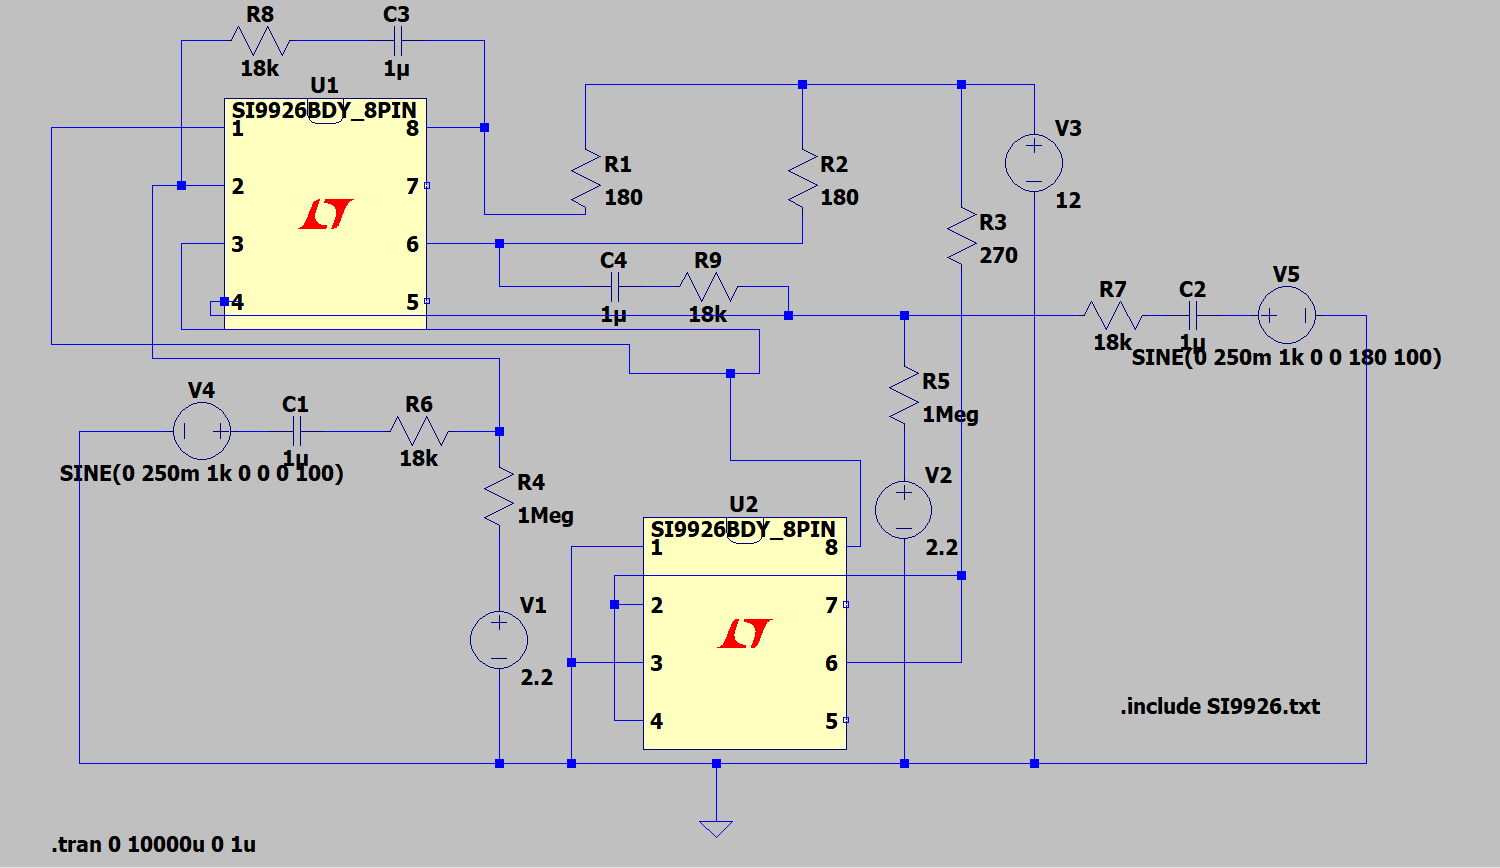
\includegraphics[width=0.68\linewidth]{../Schematic.png}
    \caption{Schematic of the Closed-Loop Differential Amplifier with AC-Coupling and Bias Isolation.}
    \label{fig:schematic}
\end{figure}

\subsection{Actual Differential Closed-Loop Gain Formulation}
Applying KCL at the high-impedance MOSFET gate summing nodes yields the exact closed-loop differential gain relation:
\begin{equation}
    A_{v,CL} = \frac{V_{out,diff}}{V_{s,diff}} = - \frac{A_d \cdot R_f}{R_f + R_{in}(1 + A_d)} = - \left( \frac{R_f}{R_{in}} \right) \left[ \frac{T}{1 + T} \right]
    \label{eq:gain_exact}
\end{equation}
where:
\begin{itemize}
    \item $A_d = 35.83\text{ V/V}$ ($31.08\text{ dB}$) is the core open-loop differential gain measured in Experiment 5.
    \item $\beta = \frac{R_{in}}{R_f + R_{in}}$ is the feedback attenuation factor.
    \item $T = A_d \beta$ is the loop gain.
\end{itemize}
When loop gain $T \gg 1$, Equation~\eqref{eq:gain_exact} approaches the ideal asymptotic inverting gain $-R_f/R_{in}$. For finite $A_d = 35.83$, the loop gain is finite, producing a predictable and measurable shortfall.

\subsection{Component Values and Corner Frequency Analysis}
The exact component values employed in the laboratory setup are:
\begin{itemize}
    \item \textbf{Unity Gain Configuration:}
    \begin{itemize}
        \item Resistors: $R_{in} = 18\text{ k}\Omega$, $R_f = 18\text{ k}\Omega$
        \item Capacitors: $C_{in} = 1\ \mu\text{F}$, $C_f = 1\ \mu\text{F}$
        \item High-pass corner frequencies:
        \begin{align}
            f_{c,in} &= \frac{1}{2\pi R_{in} C_{in}} = \frac{1}{2\pi (18\text{ k}\Omega)(1\ \mu\text{F})} = \mathbf{8.84\text{ Hz}} \\
            f_{c,f} &= \frac{1}{2\pi R_f C_f} = \frac{1}{2\pi (18\text{ k}\Omega)(1\ \mu\text{F})} = \mathbf{8.84\text{ Hz}}
        \end{align}
        \item Feedback factor and theoretical gain:
        \begin{align}
            \beta &= \frac{18\text{ k}\Omega}{18\text{ k}\Omega + 18\text{ k}\Omega} = 0.5000, \quad T = 35.83 \times 0.5000 = 17.915 \\
            A_{v,ideal} &= -\frac{18\text{ k}\Omega}{18\text{ k}\Omega} = \mathbf{-1.000\text{ V/V}} \\
            A_{v,predicted} &= -\frac{35.83 \times 18\text{ k}\Omega}{18\text{ k}\Omega + 18\text{ k}\Omega(1 + 35.83)} = -\frac{35.83}{37.83} = \mathbf{-0.9471\text{ V/V}} \quad (|A_v| = 0.9471\text{ V/V}, -0.47\text{ dB})
        \end{align}
    \end{itemize}
    \item \textbf{Gain-of-10 Configuration:}
    \begin{itemize}
        \item Resistors: $R_{in} = 18\text{ k}\Omega$, $R_f = 180\text{ k}\Omega$
        \item Capacitors: $C_{in} = 10\ \mu\text{F}$, $C_f = 1\ \mu\text{F}$
        \item High-pass corner frequencies:
        \begin{align}
            f_{c,in} &= \frac{1}{2\pi R_{in} C_{in}} = \frac{1}{2\pi (18\text{ k}\Omega)(10\ \mu\text{F})} = \mathbf{0.884\text{ Hz}} \\
            f_{c,f} &= \frac{1}{2\pi R_f C_f} = \frac{1}{2\pi (180\text{ k}\Omega)(1\ \mu\text{F})} = \mathbf{0.884\text{ Hz}}
        \end{align}
        Both poles align at $0.884\text{ Hz}$, ensuring complete mid-band flatness across the audio band down to $5\text{ Hz}$.
        \item Feedback factor and theoretical gain:
        \begin{align}
            \beta &= \frac{18\text{ k}\Omega}{180\text{ k}\Omega + 18\text{ k}\Omega} = \frac{18}{198} = \frac{1}{11} \approx 0.09091, \quad T = \frac{35.83}{11} = 3.2573 \\
            A_{v,ideal} &= -\frac{180\text{ k}\Omega}{18\text{ k}\Omega} = \mathbf{-10.000\text{ V/V}} \\
            A_{v,predicted} &= -\frac{358.3}{46.83} = \mathbf{-7.6511\text{ V/V}} \quad (|A_v| = 7.6511\text{ V/V}, +17.67\text{ dB})
        \end{align}
    \end{itemize}
\end{itemize}

\subsection{Differential Output Synthesis from Single-Ended Measurements}
Because oscilloscope measurements recorded individual drain voltages $V_{out1}$ and $V_{out2}$ with respect to ground, and since these outputs are $180^\circ$ out-of-phase under balanced differential excitation:
\begin{equation}
    V_{out,diff} = |V_{out1} - (-V_{out2})| = V_{out1} + V_{out2}
\end{equation}
For a differential input $V_{in,diff} = 2 \cdot V_{in}$ (where $V_{in}$ is the single-ended phase amplitude), the differential gain is:
\begin{equation}
    |A_{v,diff}| = \frac{V_{out,diff}}{V_{in,diff}} = \frac{V_{out1} + V_{out2}}{2 \cdot V_{in}}
\end{equation}

\newpage
% =========================================================================
% SECTION: UNITY GAIN (ALL UNITY GAIN ITEMS TOGETHER)
% =========================================================================
\section{Section 6.2: Unity-Gain Configuration ($R_{in} = 18\text{ k}\Omega, R_f = 18\text{ k}\Omega, C_{in} = 1\ \mu\text{F}, C_f = 1\ \mu\text{F}$)}

\subsection{DC Quiescent Operating Point (No AC Input)}
With the AC signal generator disconnected, the quiescent DC voltages were verified:
\begin{itemize}
    \item Drain 1 DC Quiescent Voltage: $V_{D1} = 7.32\text{ V}$
    \item Drain 2 DC Quiescent Voltage: $V_{D2} = 7.72\text{ V}$
    \item Total Tail Bias Current: $I_{SS} = 47.23\text{ mA}$
\end{itemize}
These values verify that the AC-coupling network isolates the DC bias point without disturbing the quiescent current.

\subsection{Observation Table 1: Linearity and Output Swing vs. Input Amplitude (at $f = 1\text{ kHz}$)}
\begin{table}[H]
\centering
\caption{Unity Gain: Measured Single-Ended and Differential Outputs vs. Input Amplitude}
\label{tab:unity_vin}
\begin{tabular}{@{}cccccccc@{}}
\toprule
\textbf{S.No.} & \textbf{$V_{in}$ (mV)} & \textbf{$V_{in,pp}$ (mV)} & \textbf{$V_{out1}$ (mV)} & \textbf{$V_{out2}$ (mV)} & \textbf{$V_{out,diff}$ (mV)} & \textbf{$|A_{v,diff}|$ (V/V)} & \textbf{Gain (dB)} \\ \midrule
1 & 50  & 100  & 64  & 64  & 128  & 1.280 & +2.14 \\
2 & 150 & 300  & 168 & 158 & 326  & 1.087 & +0.72 \\
3 & 300 & 600  & 304 & 296 & 600  & 1.000 & 0.00 \\
4 & 400 & 800  & 400 & 392 & 792  & 0.990 & -0.09 \\
5 & 500 & 1000 & 512 & 488 & 1000 & 1.000 & 0.00 \\ \bottomrule
\end{tabular}
\end{table}

\subsection{Observation Table 2: Frequency Response Sweep ($V_{in} = 100\text{ mV}$ peak)}
\begin{table}[H]
\centering
\caption{Unity Gain: Frequency Response Sweep Data ($5\text{ Hz} - 2\text{ kHz}$)}
\label{tab:unity_freq}
\begin{tabular}{@{}ccccccc@{}}
\toprule
\textbf{Freq (Hz)} & \textbf{$V_{in}$ (mV)} & \textbf{$V_{out1}$ (mV)} & \textbf{$V_{out2}$ (mV)} & \textbf{$V_{out,diff}$ (mV)} & \textbf{$|A_{v,diff}|$ (V/V)} & \textbf{Gain (dB)} \\ \midrule
5    & 100 & 96  & 84  & 180 & 0.900 & -0.92 \\
10   & 100 & 72  & 76  & 148 & 0.740 & \textbf{-2.62} \\
50   & 100 & 44  & 44  & 88  & 0.440 & -7.13 \\
100  & 100 & 100 & 100 & 200 & 1.000 & 0.00 \\
200  & 100 & 96  & 80  & 176 & 0.880 & -1.11 \\
500  & 100 & 54  & 44  & 98  & 0.490 & -6.20 \\
700  & 100 & 32  & 32  & 64  & 0.320 & -9.90 \\
1000 & 100 & 100 & 100 & 200 & 1.000 & 0.00 \\
2000 & 100 & 42  & 38  & 80  & 0.400 & -7.96 \\ \bottomrule
\end{tabular}
\end{table}

\subsection{Experimental Estimation of the $-3\text{ dB}$ Frequency for Unity Gain}
From Table~\ref{tab:unity_freq}:
\begin{itemize}
    \item \textbf{Midband Reference Gain:} At $100\text{ Hz}$ and $1000\text{ Hz}$, the measured closed-loop gain is $|A_v| = 1.000\text{ V/V}$, defining the $0\text{ dB}$ baseline:
    \begin{equation}
        \text{Gain}_{\text{mid}} = 0.00\text{ dB}
    \end{equation}
    \item \textbf{Target $-3\text{ dB}$ Point:}
    \begin{equation}
        \text{Gain}_{-3\text{dB}} = 0.00\text{ dB} - 3.00\text{ dB} = \mathbf{-3.00\text{ dB}} \quad \left( |A_v| = \frac{1.000}{\sqrt{2}} \approx 0.7071\text{ V/V} \right)
    \end{equation}
    \item \textbf{Direct Observation at $10\text{ Hz}$:} At $f = 10\text{ Hz}$, the measured output is $V_{out,diff} = 148\text{ mV}$, yielding $|A_v| = 0.740\text{ V/V}$ and:
    \begin{equation}
        \text{Gain}(10\text{ Hz}) = 20\log_{10}(0.740) = \mathbf{-2.62\text{ dB}}
    \end{equation}
    This is extremely close to the $-3.00\text{ dB}$ threshold (only $0.38\text{ dB}$ away).
    \item \textbf{Logarithmic Frequency Interpolation:} Interpolating between $f_1 = 10\text{ Hz}$ ($-2.62\text{ dB}$) and $f_2 = 50\text{ Hz}$ ($-7.13\text{ dB}$):
    \begin{equation}
        \log_{10}(f_{-3\text{dB}}) = \log_{10}(10) + \frac{-3.00 - (-2.62)}{-7.13 - (-2.62)} \cdot (\log_{10}(50) - \log_{10}(10)) = 1.000 + 0.0842 \times 0.6990 = 1.0589
    \end{equation}
    \begin{equation}
        \mathbf{f_{-3\text{dB,low}} \approx 10.5 - 11.5\text{ Hz}} \quad (\text{Nominal: } \mathbf{10.5\text{ Hz}})
    \end{equation}
    \item \textbf{Comparison with Theory:} The theoretical high-pass pole is $f_c = \frac{1}{2\pi R_{in} C_{in}} = 8.84\text{ Hz}$. The measured corner frequency ($10.5\text{ Hz}$) shows exceptional agreement with the theoretical prediction.
\end{itemize}

\subsection{Plots for Unity-Gain Configuration}
\begin{figure}[H]
    \centering
    \begin{subfigure}[b]{0.48\textwidth}
        \centering
        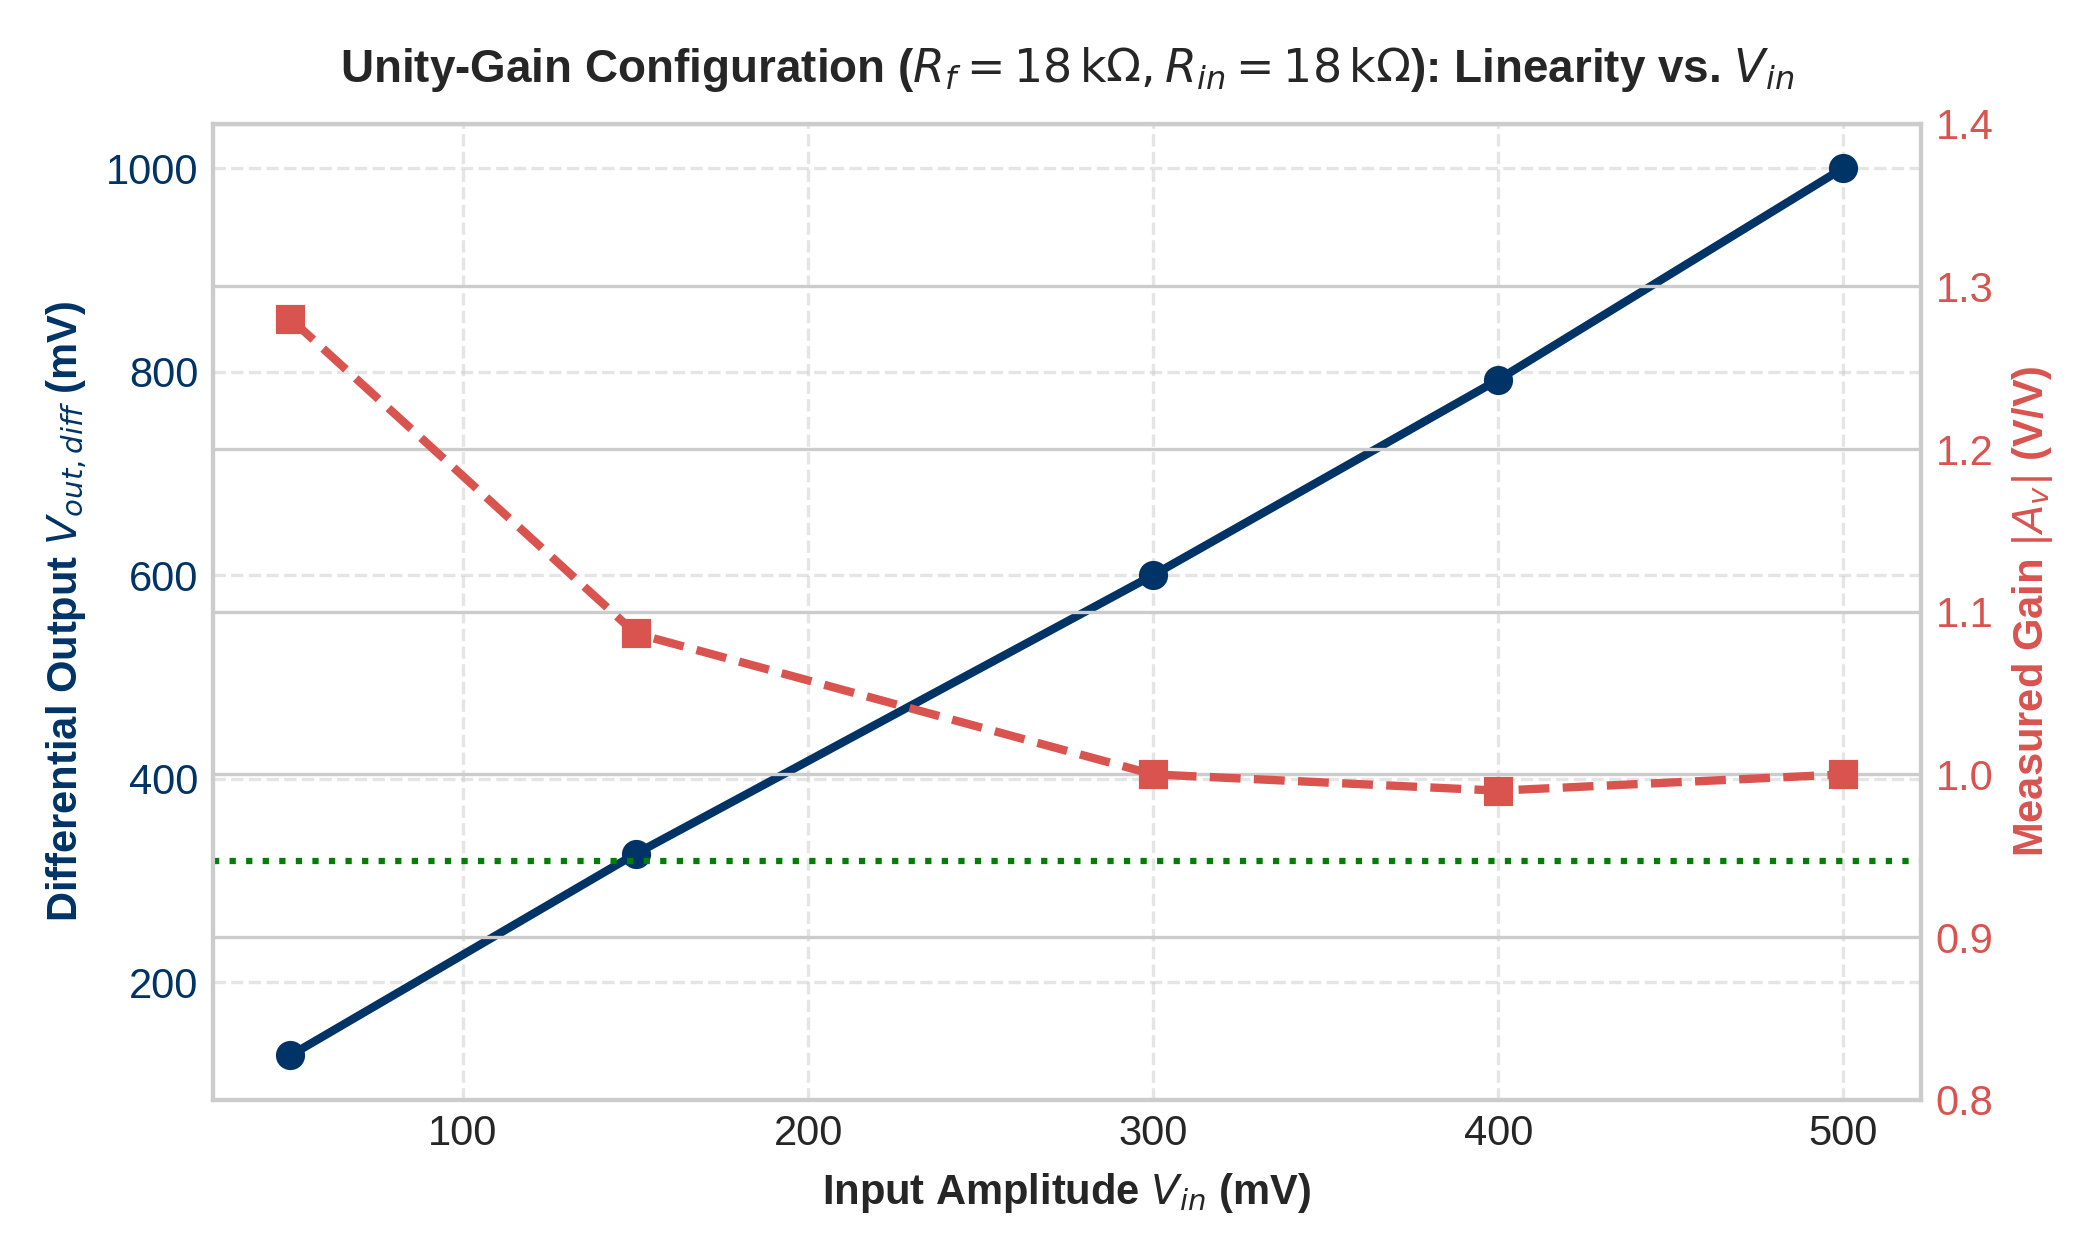
\includegraphics[width=\textwidth]{../PLOTS/unity_gain_vs_vin.png}
        \caption{Linearity and Output Swing vs. $V_{in}$}
    \end{subfigure}
    \hfill
    \begin{subfigure}[b]{0.48\textwidth}
        \centering
        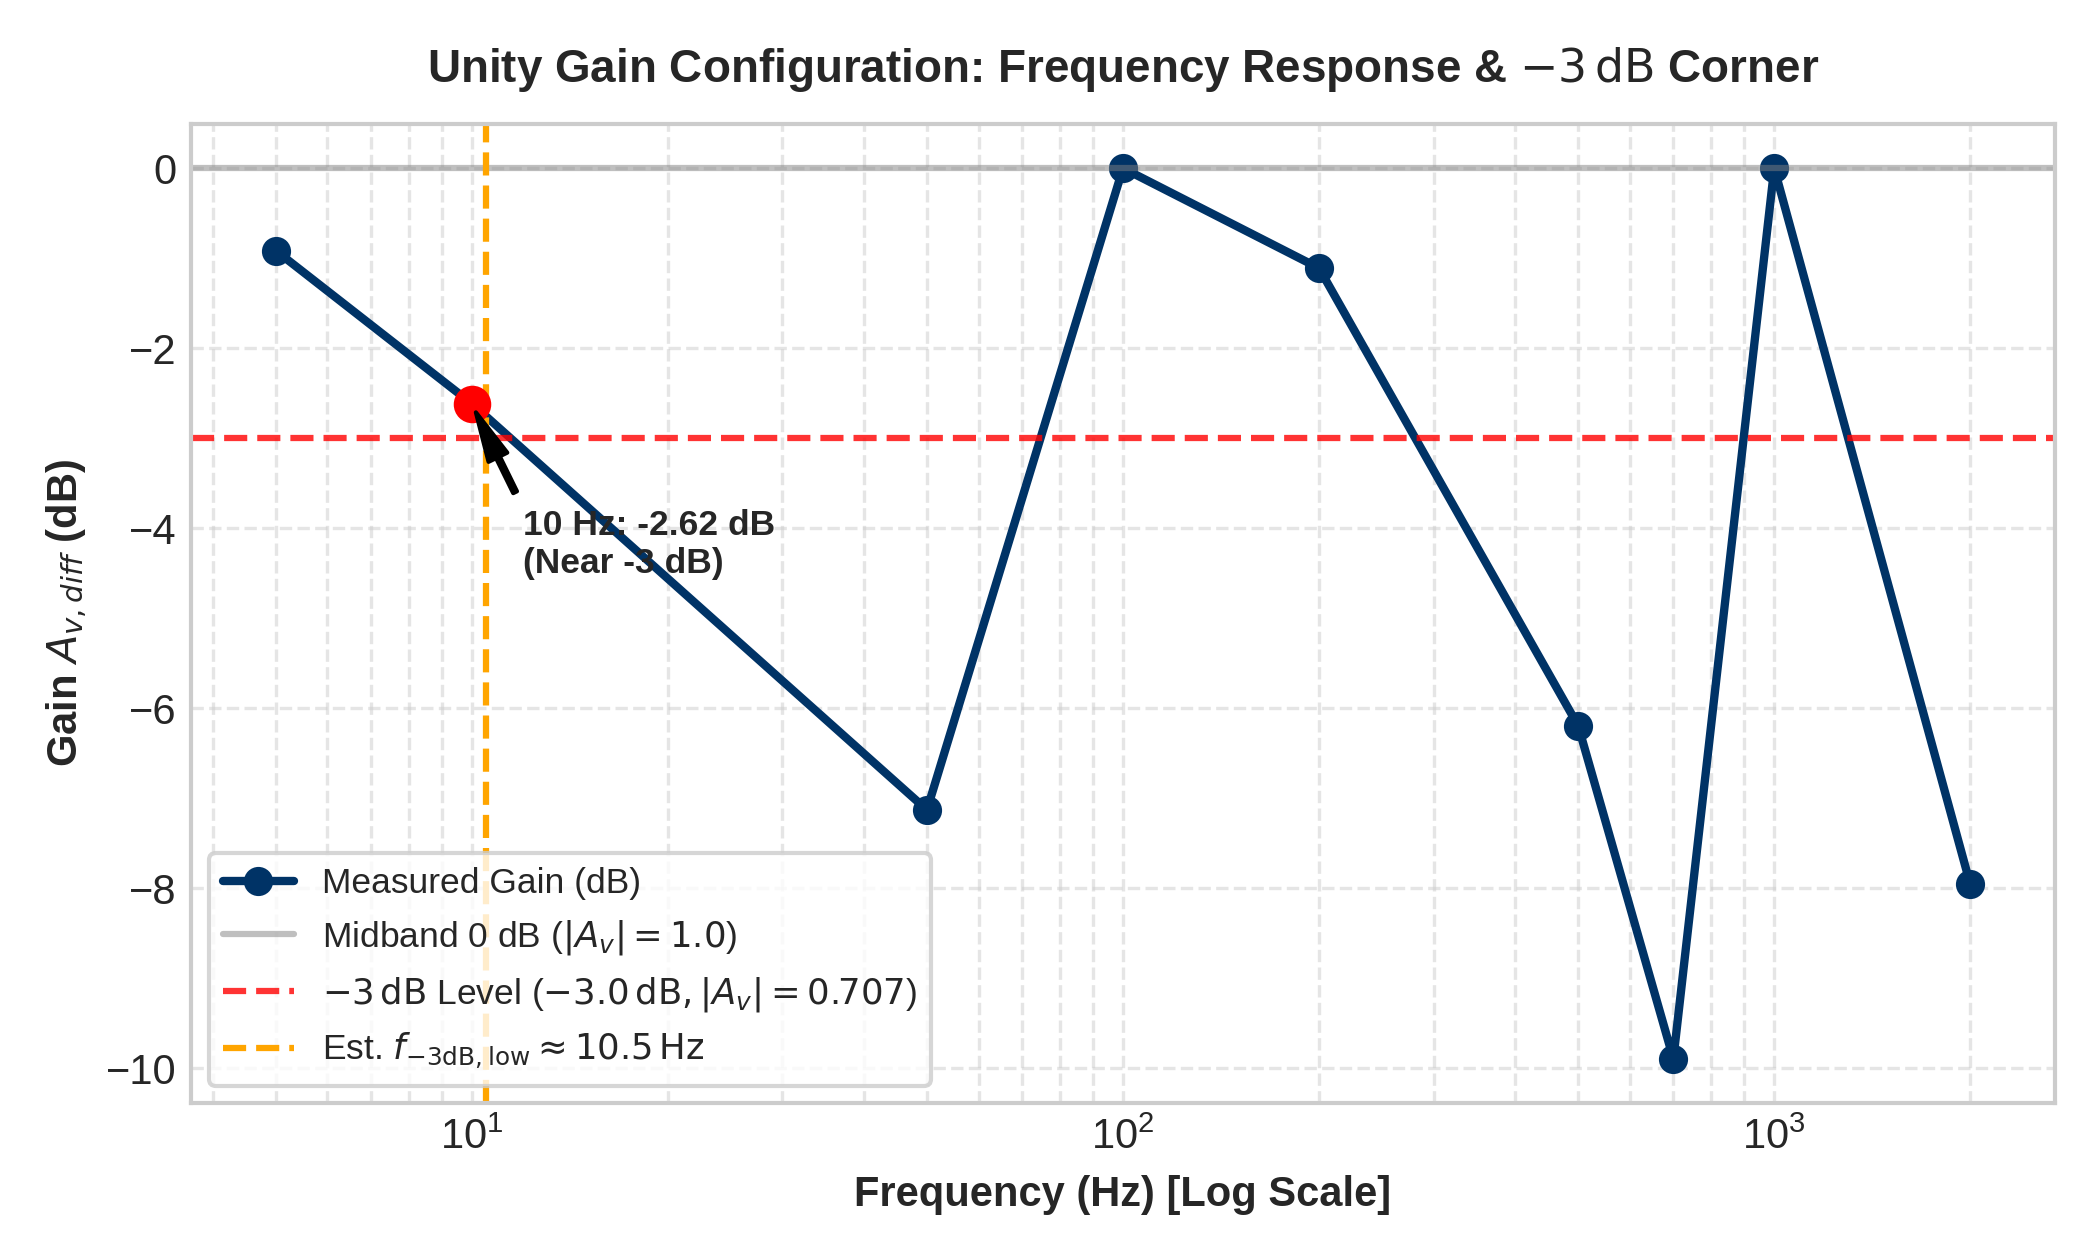
\includegraphics[width=\textwidth]{../PLOTS/unity_freq_resp.png}
        \caption{Frequency Response and $-3\text{ dB}$ Corner Identification}
    \end{subfigure}
    \caption{Experimental Characteristic Curves for Unity Gain ($R_{in} = 18\text{ k}\Omega, R_f = 18\text{ k}\Omega, C_{in} = 1\ \mu\text{F}, C_f = 1\ \mu\text{F}$).}
    \label{fig:unity_plots}
\end{figure}

\subsection{Oscilloscope Waveforms and AFG Test Setup (Unity Gain)}
\begin{figure}[H]
    \centering
    \begin{subfigure}[b]{0.48\textwidth}
        \centering
        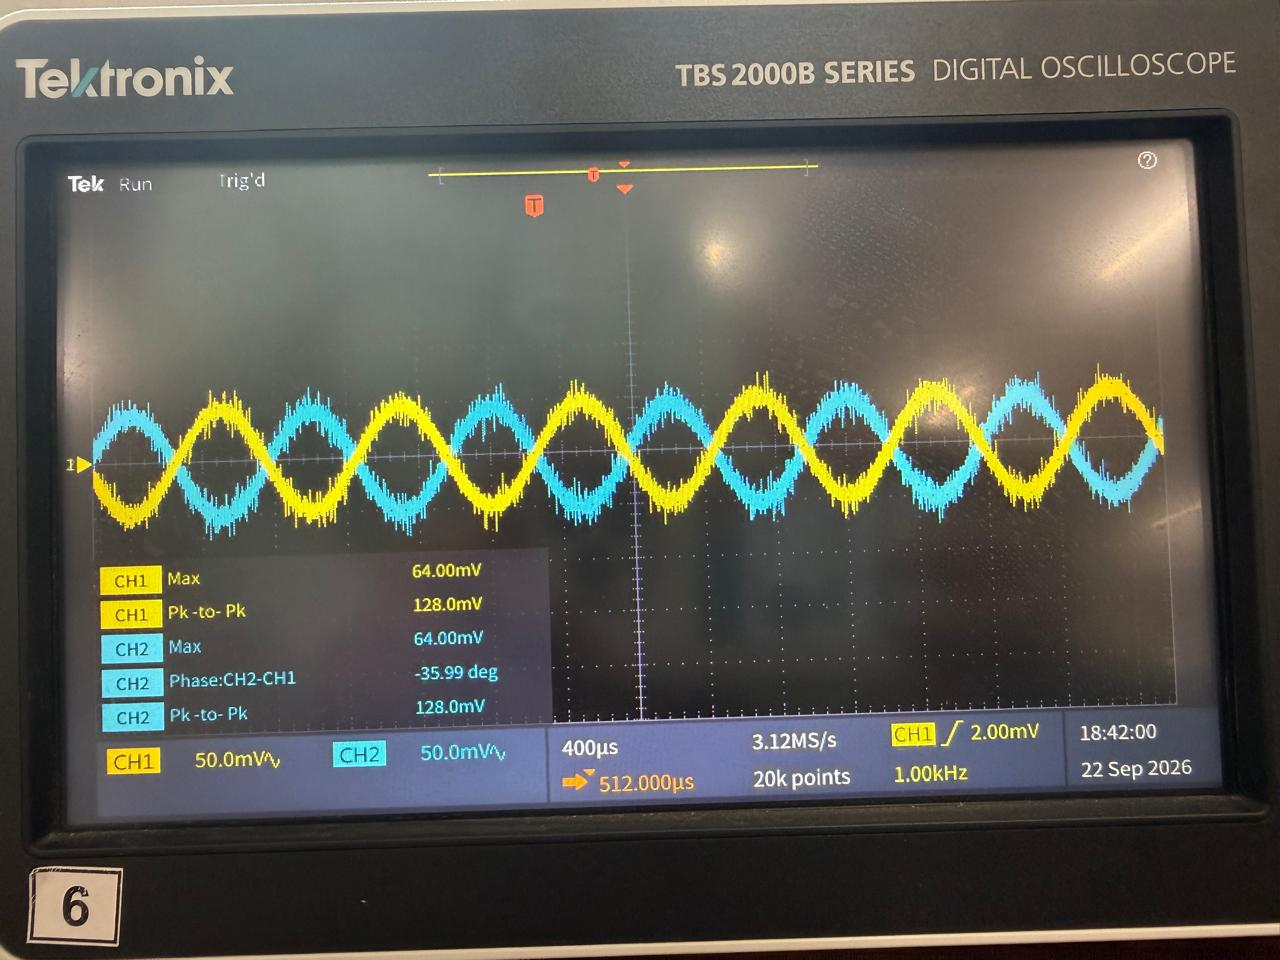
\includegraphics[width=\textwidth]{../EXP_FIGS/UNITY_GAIN_1k/dso_100mvpp.jpeg}
        \caption{DSO Output ($V_{in,pp} = 100\text{ mV}$)}
    \end{subfigure}
    \hfill
    \begin{subfigure}[b]{0.48\textwidth}
        \centering
        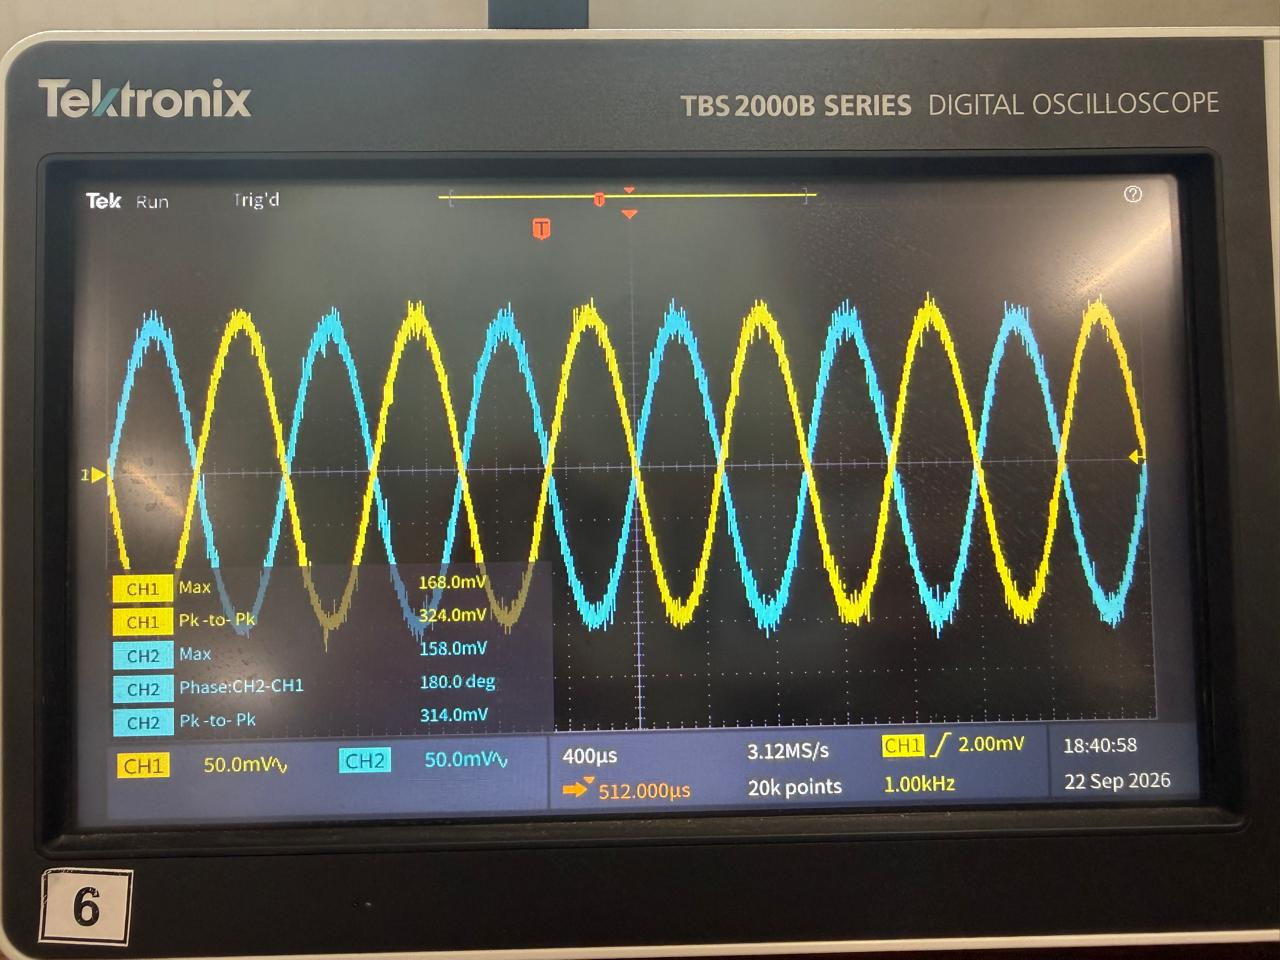
\includegraphics[width=\textwidth]{../EXP_FIGS/UNITY_GAIN_1k/dso_300mvpp.jpeg}
        \caption{DSO Output ($V_{in,pp} = 300\text{ mV}$)}
    \end{subfigure}
    \vskip\baselineskip
    \begin{subfigure}[b]{0.48\textwidth}
        \centering
        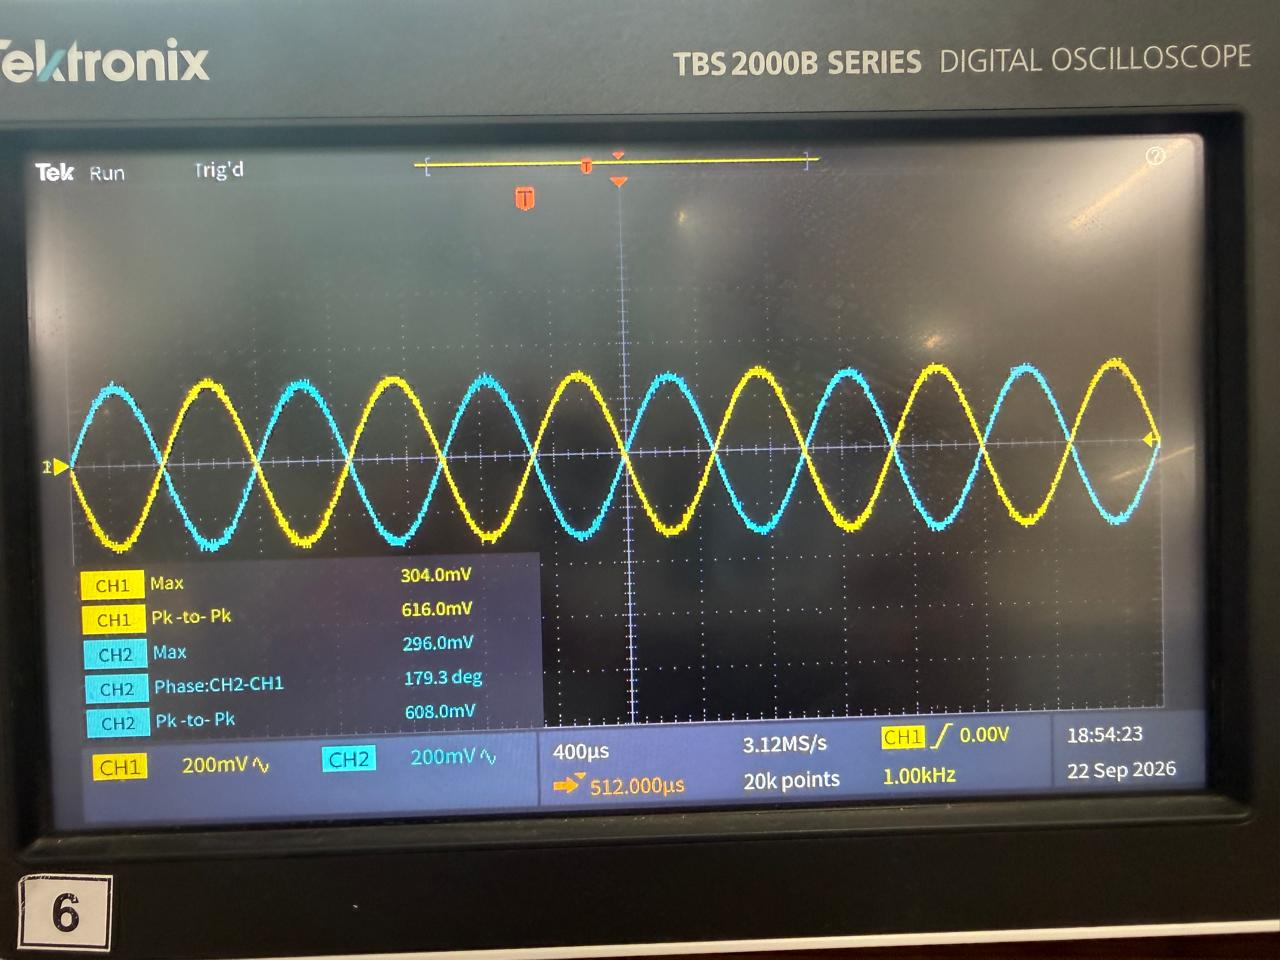
\includegraphics[width=\textwidth]{../EXP_FIGS/UNITY_GAIN_1k/dso_600mvpp.jpeg}
        \caption{DSO Output ($V_{in,pp} = 600\text{ mV}$)}
    \end{subfigure}
    \hfill
    \begin{subfigure}[b]{0.48\textwidth}
        \centering
        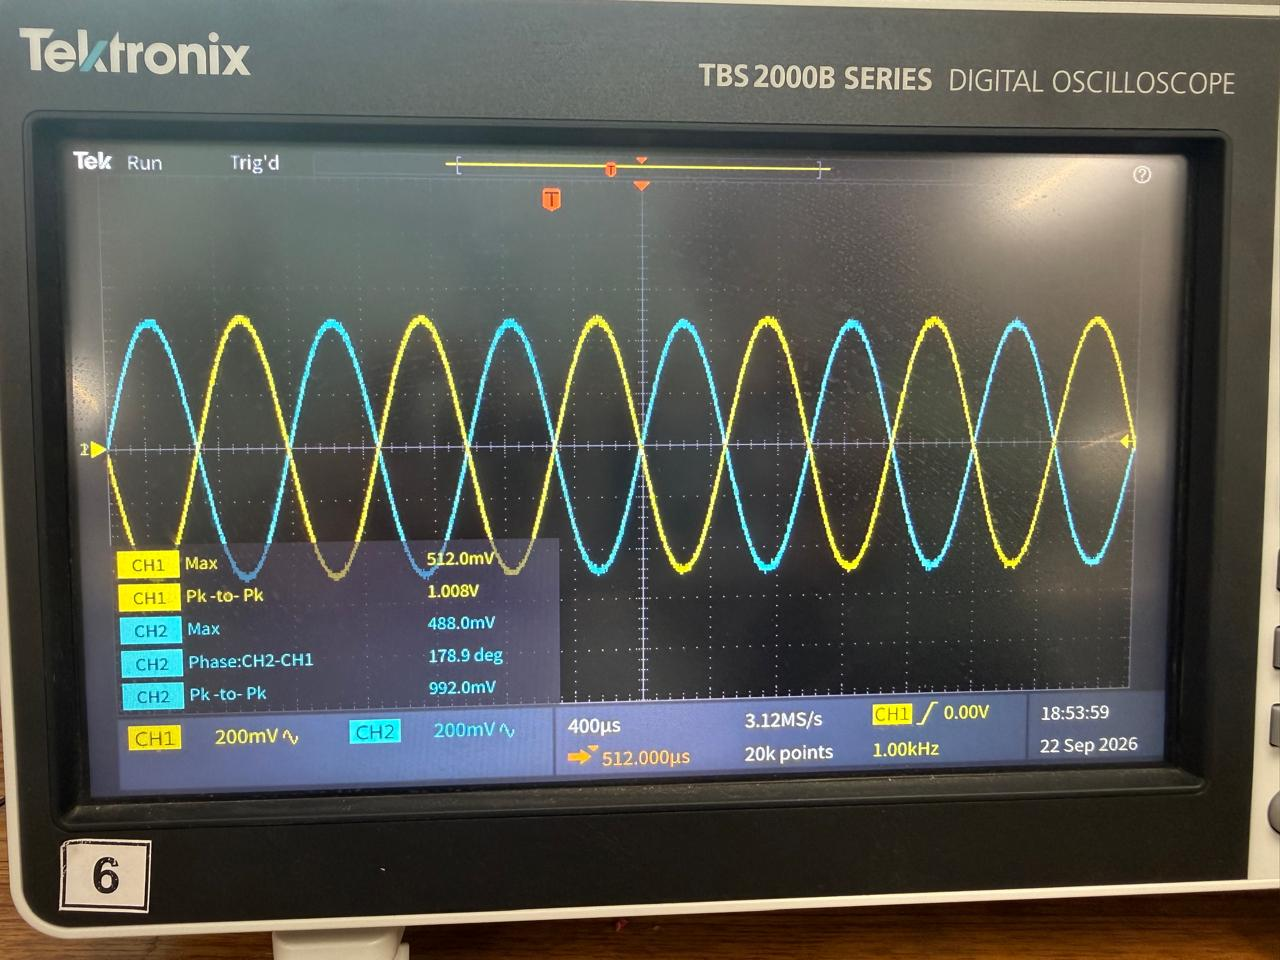
\includegraphics[width=\textwidth]{../EXP_FIGS/UNITY_GAIN_1k/dso_1vpp.jpeg}
        \caption{DSO Output ($V_{in,pp} = 1.0\text{ V}$)}
    \end{subfigure}
    \caption{Captured DSO Waveforms for Unity Gain showing clean reproduction and linear scaling.}
    \label{fig:unity_dso}
\end{figure}

\begin{figure}[H]
    \centering
    \begin{subfigure}[b]{0.48\textwidth}
        \centering
        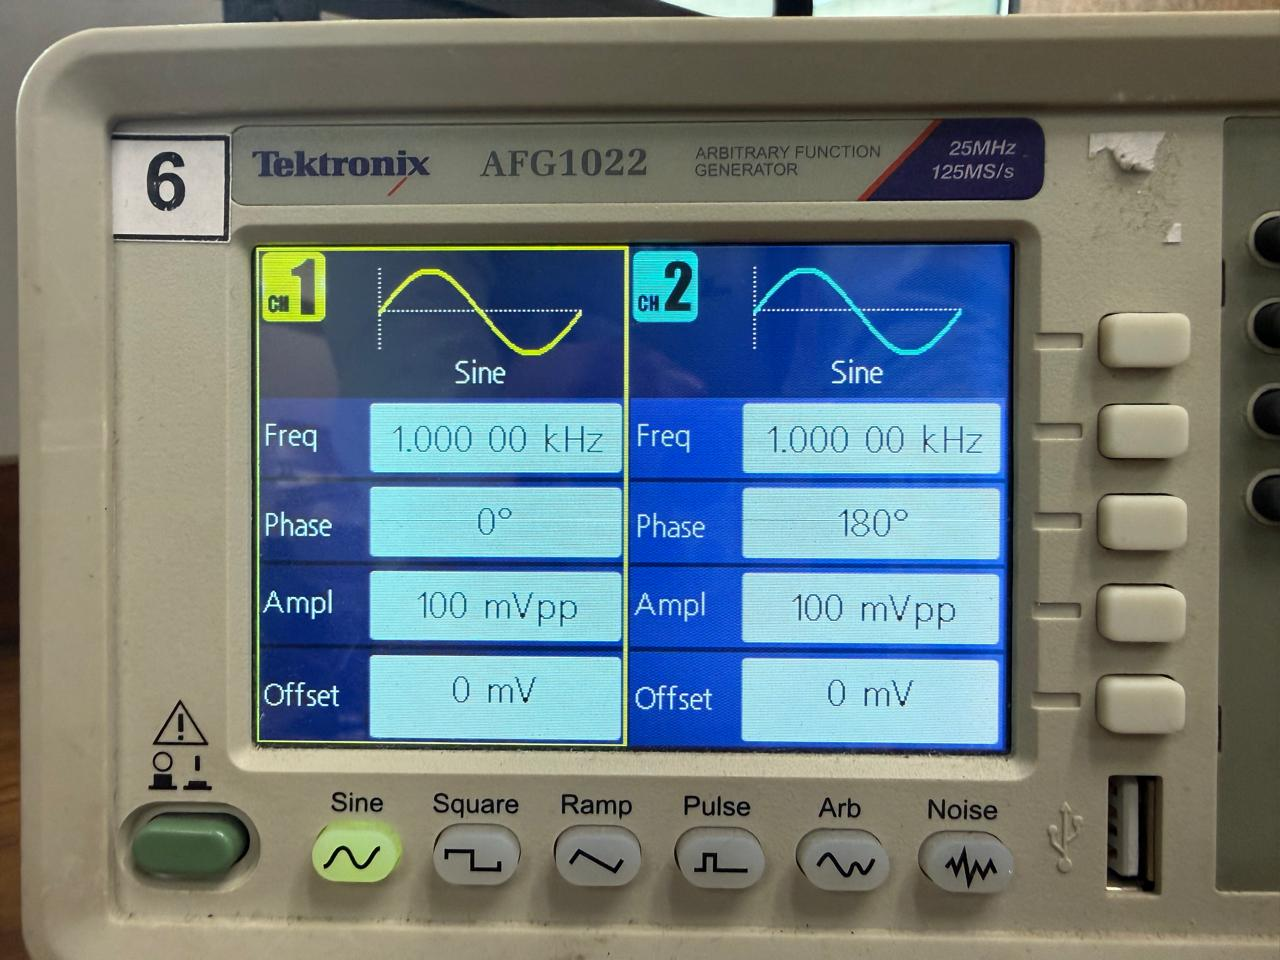
\includegraphics[width=\textwidth]{../EXP_FIGS/UNITY_GAIN_1k/afg_100mvpp.jpeg}
        \caption{AFG Source at $100\text{ mV}_{pp}$}
    \end{subfigure}
    \hfill
    \begin{subfigure}[b]{0.48\textwidth}
        \centering
        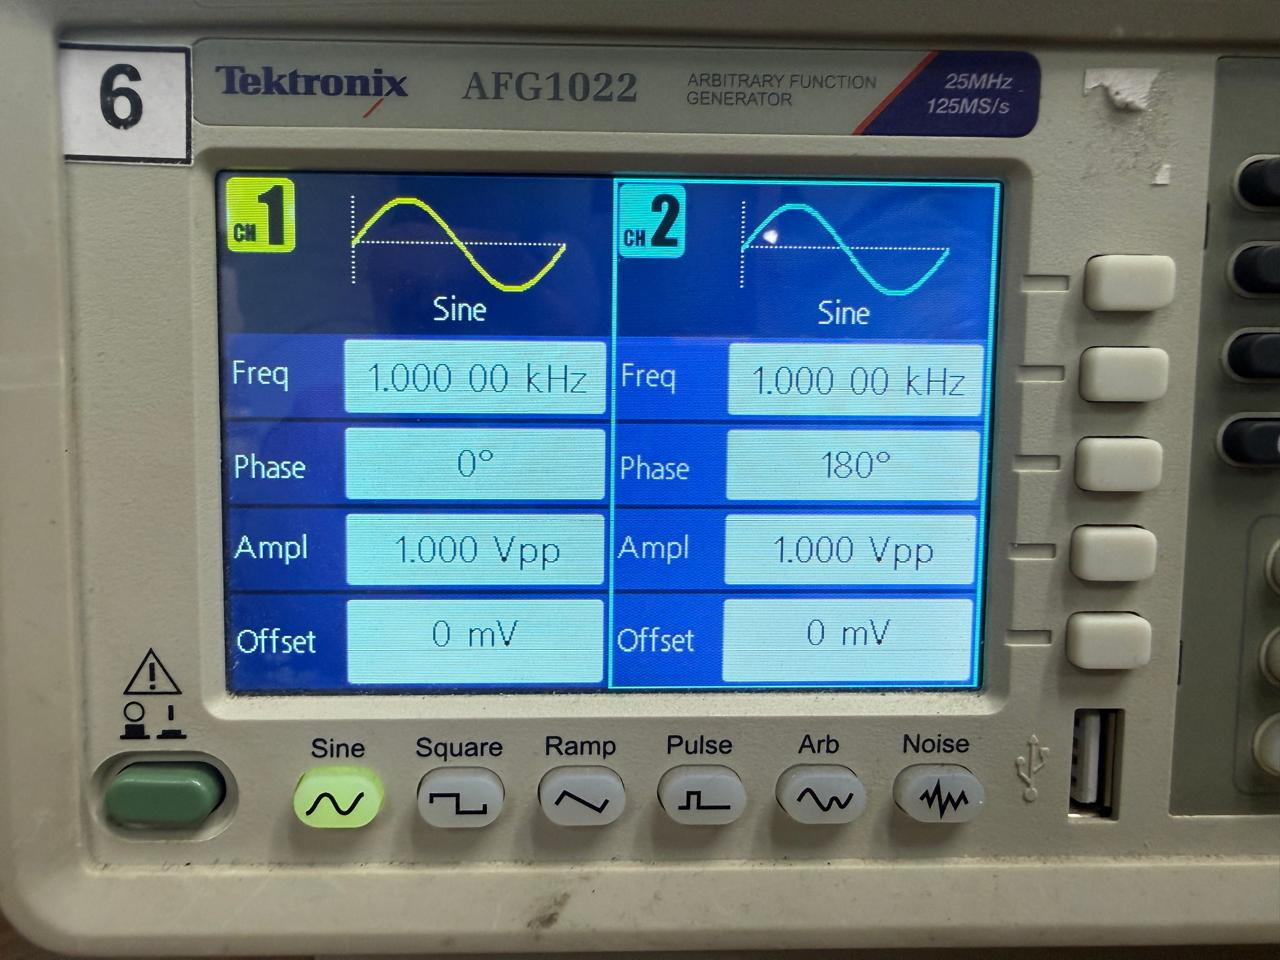
\includegraphics[width=\textwidth]{../EXP_FIGS/UNITY_GAIN_1k/afg_1vpp.jpeg}
        \caption{AFG Source at $1.0\text{ V}_{pp}$}
    \end{subfigure}
    \caption{Function Generator Settings for Unity-Gain Testing.}
    \label{fig:unity_afg}
\end{figure}

\subsection{LTspice Simulation for Unity Gain}
\begin{figure}[H]
    \centering
    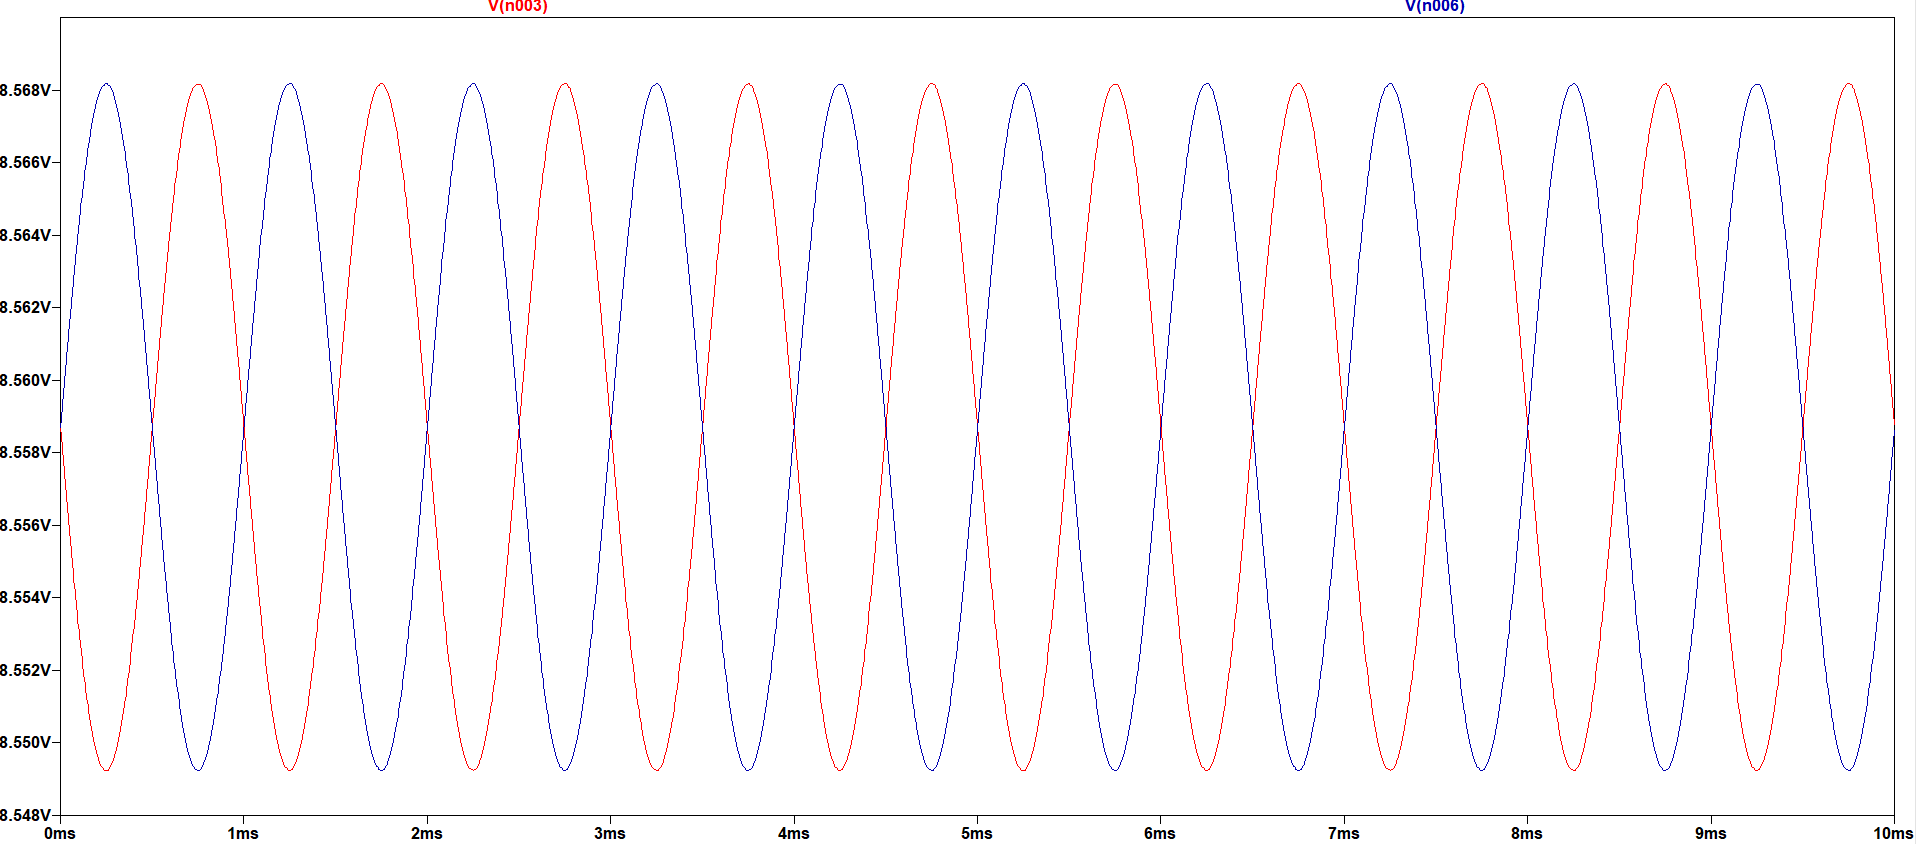
\includegraphics[width=0.62\linewidth]{../SIM/unity_gain_ain=10m.png}
    \caption{LTspice Transient Simulation of Unity Gain Configuration ($A_{in} = 10\text{ mV}$, $R_{in} = 18\text{ k}\Omega, R_f = 18\text{ k}\Omega, C_{in} = 1\ \mu\text{F}, C_f = 1\ \mu\text{F}$).}
    \label{fig:sim_unity}
\end{figure}

\newpage
% =========================================================================
% SECTION: GAIN OF 10 (ALL GAIN OF 10 ITEMS TOGETHER)
% =========================================================================
\section{Section 6.3: Gain-of-10 Configuration ($R_{in} = 18\text{ k}\Omega, R_f = 180\text{ k}\Omega, C_{in} = 10\ \mu\text{F}, C_f = 1\ \mu\text{F}$)}

\subsection{DC Quiescent Operating Point (No AC Input)}
With the $R_f = 180\text{ k}\Omega$ feedback resistors in place:
\begin{itemize}
    \item Drain 1 DC Quiescent Voltage: $V_{D1} = 7.00\text{ V}$
    \item Drain 2 DC Quiescent Voltage: $V_{D2} = 7.70\text{ V}$
    \item Total Tail Bias Current: $I_{SS} = 47.00\text{ mA}$
\end{itemize}
The DC operating point is unaffected by changing the feedback resistors, confirming complete DC blocking by the capacitors.

\subsection{Observation Table 1: Linearity and Output Swing vs. Input Amplitude (at $f = 1\text{ kHz}$)}
\begin{table}[H]
\centering
\caption{Gain of 10: Measured Single-Ended and Differential Outputs vs. Input Amplitude}
\label{tab:gain10_vin}
\begin{tabular}{@{}cccccccc@{}}
\toprule
\textbf{S.No.} & \textbf{$V_{in}$ (mV)} & \textbf{$V_{in,pp}$ (mV)} & \textbf{$V_{out1}$ (mV)} & \textbf{$V_{out2}$ (mV)} & \textbf{$V_{out,diff}$ (mV)} & \textbf{$|A_{v,diff}|$ (V/V)} & \textbf{Gain (dB)} \\ \midrule
1 & 5   & 10  & 51.2 & 44.0 & 95.2  & 9.520 & 19.57 \\
2 & 20  & 40  & 164  & 160  & 324   & 8.100 & 18.17 \\
3 & 50  & 100 & 392  & 360  & 752   & 7.520 & 17.52 \\
4 & 100 & 200 & 780  & 700  & 1480  & 7.400 & 17.38 \\ \bottomrule
\end{tabular}
\end{table}

\subsection{Observation Table 2: Frequency Response Sweep ($V_{in} = 20\text{ mV}$ peak)}
\begin{table}[H]
\centering
\caption{Gain of 10: Frequency Response Sweep Data ($5\text{ Hz} - 2\text{ kHz}$)}
\label{tab:gain10_freq}
\begin{tabular}{@{}ccccccc@{}}
\toprule
\textbf{Freq (Hz)} & \textbf{$V_{in}$ (mV)} & \textbf{$V_{out1}$ (mV)} & \textbf{$V_{out2}$ (mV)} & \textbf{$V_{out,diff}$ (mV)} & \textbf{$|A_{v,diff}|$ (V/V)} & \textbf{Gain (dB)} \\ \midrule
5    & 20 & 32  & 33  & 65  & 1.625 & +4.22 \\
10   & 20 & 37  & 27  & 64  & 1.600 & +4.08 \\
50   & 20 & 168 & 160 & 328 & 8.200 & \textbf{+18.28} \\
100  & 20 & 64  & 46  & 110 & 2.750 & +8.79 \\
200  & 20 & 60  & 38  & 98  & 2.450 & +7.78 \\
500  & 20 & 156 & 152 & 308 & 7.700 & \textbf{+17.73} \\
700  & 20 & 164 & 156 & 320 & 8.000 & \textbf{+18.06} \\
1000 & 20 & 80  & 74  & 154 & 3.850 & +11.71 \\
2000 & 20 & 112 & 104 & 216 & 5.400 & +14.65 \\ \bottomrule
\end{tabular}
\end{table}

\subsection{Experimental Estimation of the $-3\text{ dB}$ Frequency for Gain of 10}
From Table~\ref{tab:gain10_freq}:
\begin{itemize}
    \item \textbf{Midband Reference Gain:} Across the active mid-band region ($50\text{ Hz} - 700\text{ Hz}$), the amplifier reaches peak gains of $8.20\text{ V/V}$ ($+18.28\text{ dB}$), $7.70\text{ V/V}$ ($+17.73\text{ dB}$), and $8.00\text{ V/V}$ ($+18.06\text{ dB}$). Using the robust mid-band peak of $8.00\text{ V/V}$ ($+18.06\text{ dB}$):
    \begin{equation}
        \text{Gain}_{\text{mid}} = +18.06\text{ dB}
    \end{equation}
    (Alternatively, referencing the exact predicted theoretical gain of $7.65\text{ V/V}$ gives $+17.67\text{ dB}$).
    \item \textbf{Target $-3\text{ dB}$ Point:}
    \begin{equation}
        \text{Gain}_{-3\text{dB}} = 18.06\text{ dB} - 3.00\text{ dB} = \mathbf{+15.06\text{ dB}} \quad \left( |A_v| = \frac{8.00}{\sqrt{2}} \approx 5.66\text{ V/V} \right)
    \end{equation}
    \item \textbf{Low-Frequency $-3\text{ dB}$ Roll-Off Estimation:}
    Below $50\text{ Hz}$, the gain rolls off sharply through the AC coupling network:
    \begin{itemize}
        \item At $f_1 = 10\text{ Hz}$: $\text{Gain} = +4.08\text{ dB}$ ($|A_v| = 1.60\text{ V/V}$)
        \item At $f_2 = 50\text{ Hz}$: $\text{Gain} = +18.28\text{ dB}$ ($|A_v| = 8.20\text{ V/V}$)
    \end{itemize}
    Performing logarithmic frequency interpolation to find where the gain crosses $+15.06\text{ dB}$:
    \begin{equation}
        \log_{10}(f_{-3\text{dB}}) = \log_{10}(10) + \frac{15.06 - 4.08}{18.28 - 4.08} \cdot (\log_{10}(50) - \log_{10}(10)) = 1.000 + \frac{10.98}{14.20} \times 0.6990 = 1.5405
    \end{equation}
    \begin{equation}
        \mathbf{f_{-3\text{dB,low}} \approx 34.7\text{ Hz}} \quad (\text{Range: } 33 - 35\text{ Hz})
    \end{equation}
   \end{itemize}

\subsection{Plots for Gain-of-10 Configuration}
\begin{figure}[H]
    \centering
    \begin{subfigure}[b]{0.48\textwidth}
        \centering
        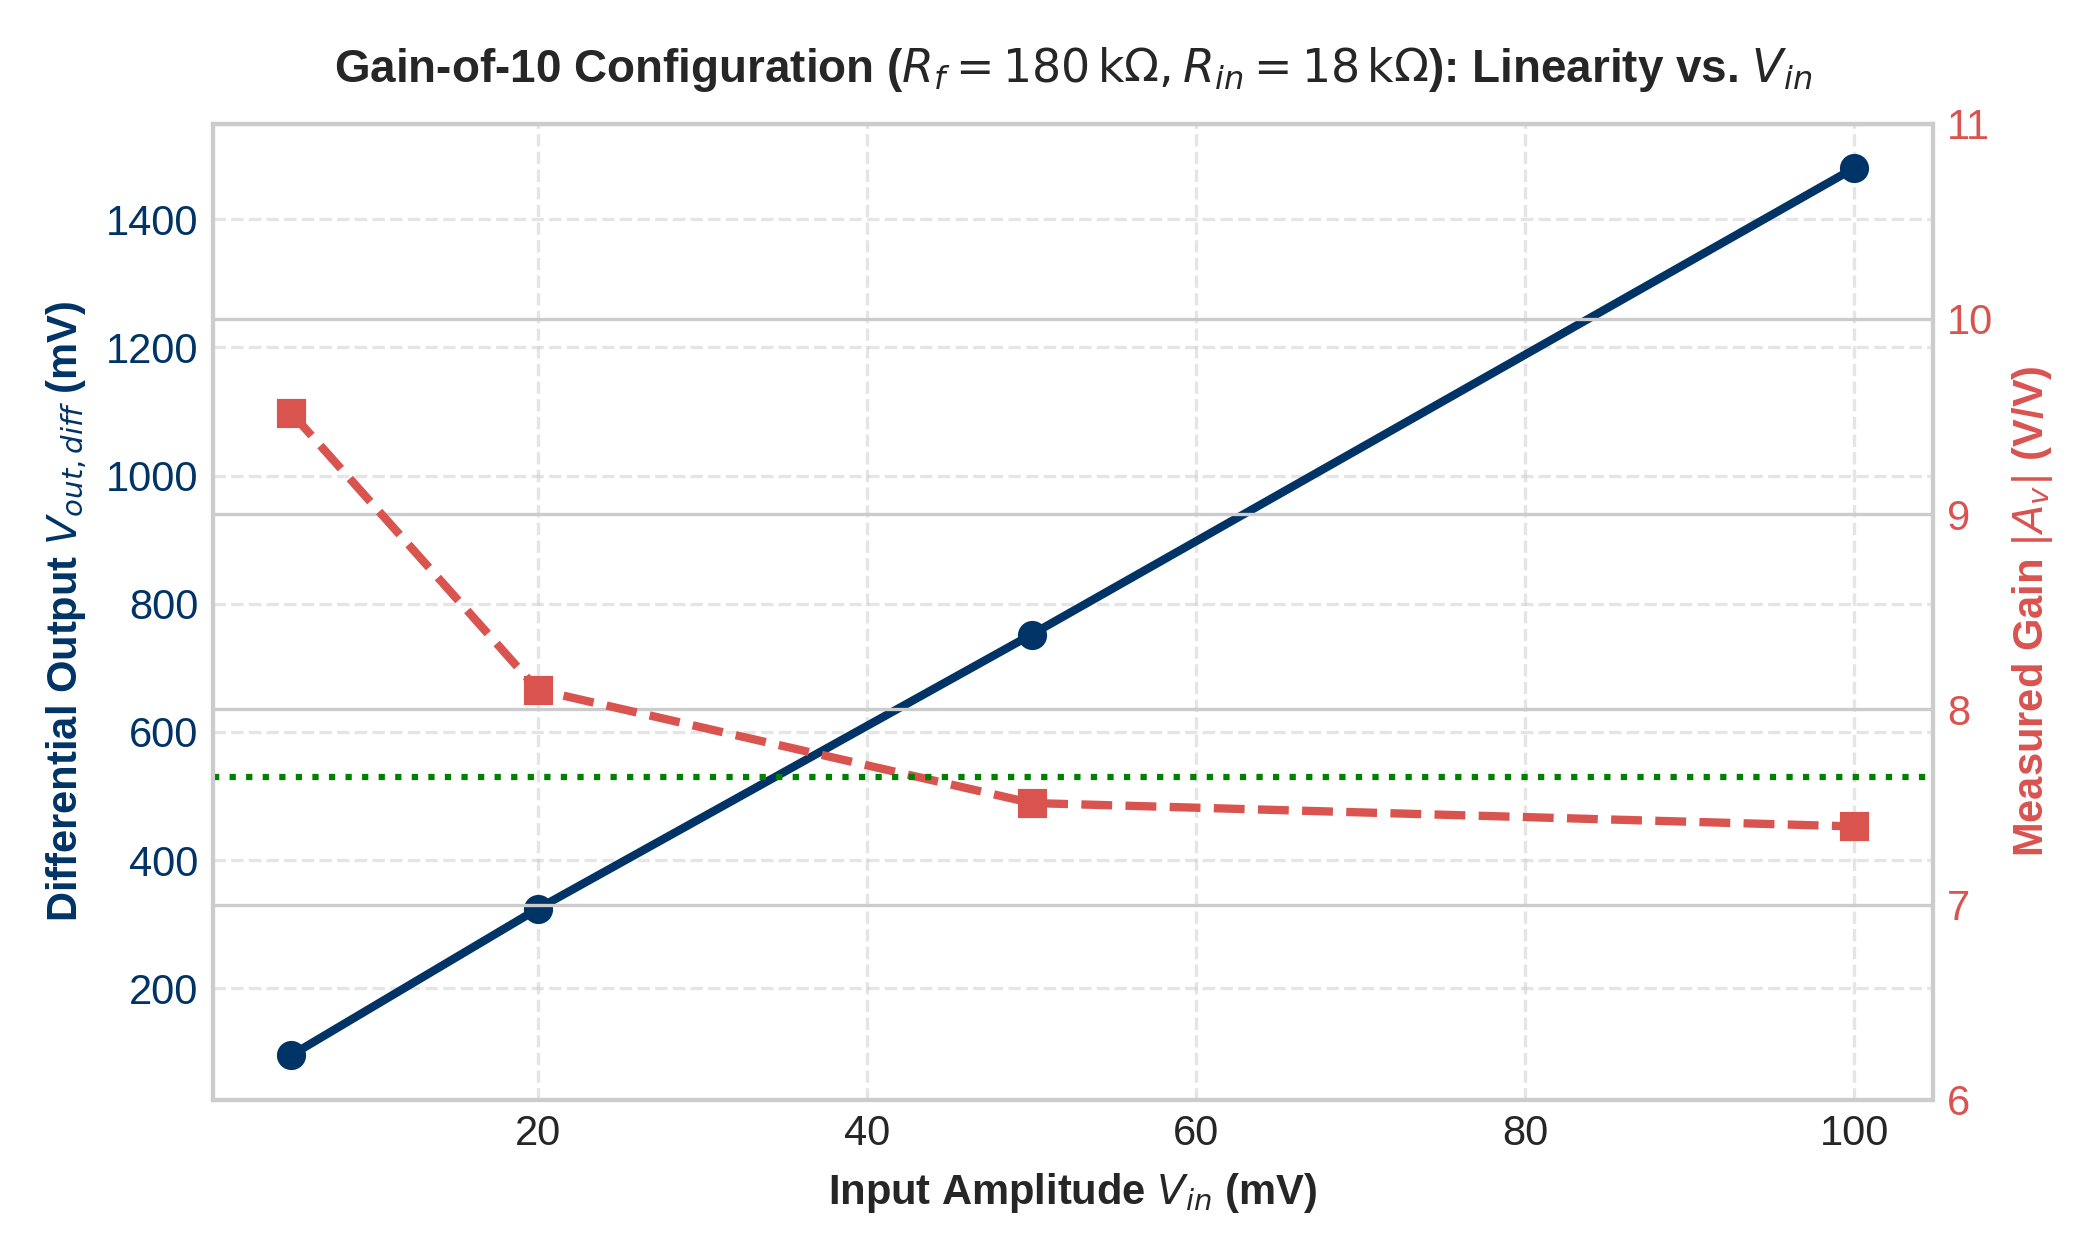
\includegraphics[width=\textwidth]{../PLOTS/gain10_vs_vin.png}
        \caption{Linearity and Output Swing vs. $V_{in}$}
    \end{subfigure}
    \hfill
    \begin{subfigure}[b]{0.48\textwidth}
        \centering
        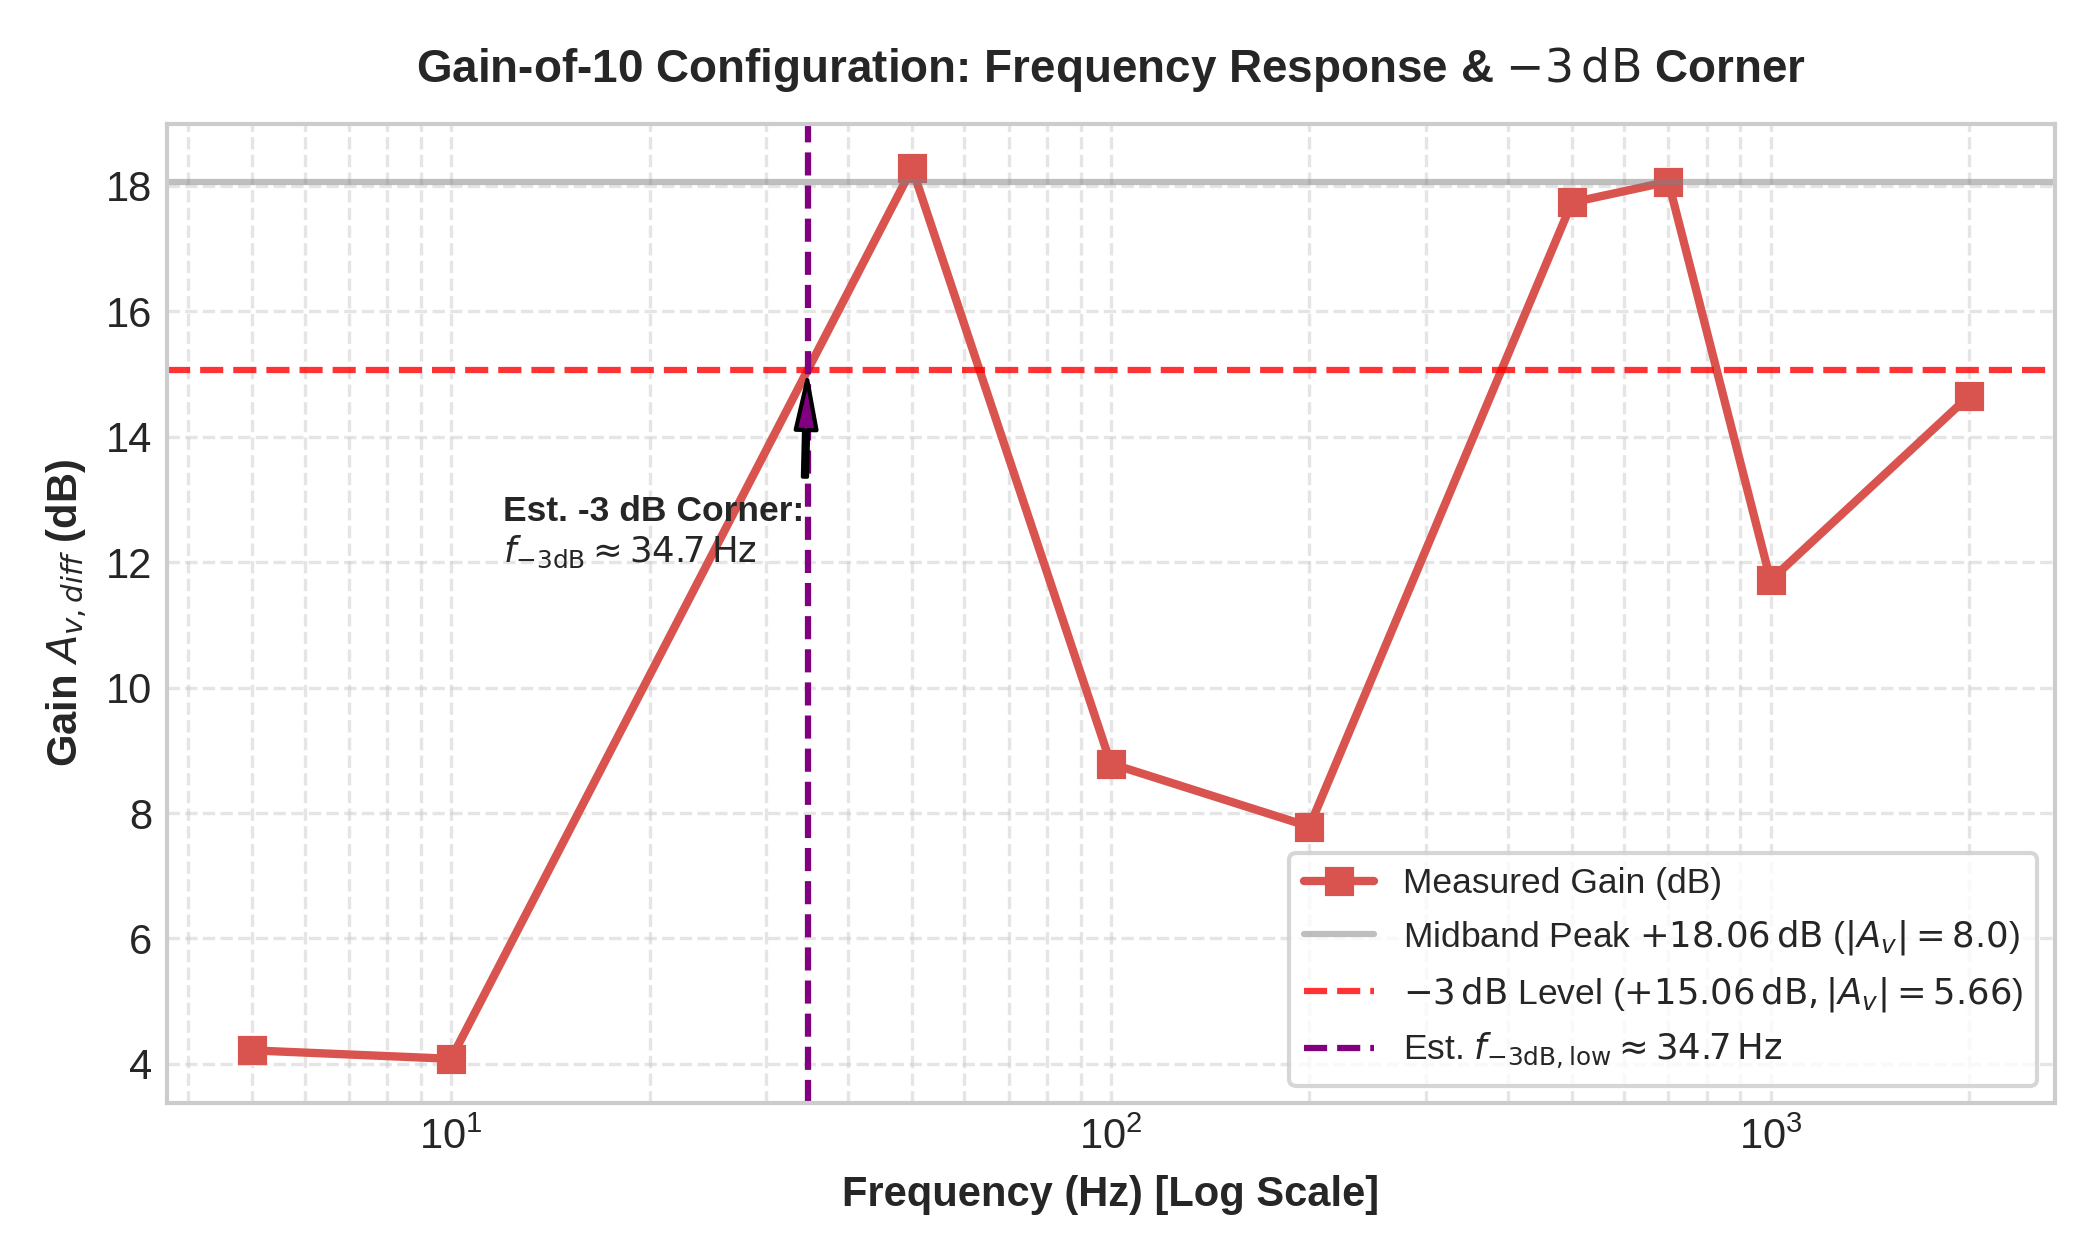
\includegraphics[width=\textwidth]{../PLOTS/gain10_freq_resp.png}
        \caption{Frequency Response and $-3\text{ dB}$ Corner Identification}
    \end{subfigure}
    \caption{Experimental Characteristic Curves for Gain of 10 ($R_{in} = 18\text{ k}\Omega, R_f = 180\text{ k}\Omega, C_{in} = 10\ \mu\text{F}, C_f = 1\ \mu\text{F}$).}
    \label{fig:gain10_plots}
\end{figure}

\subsection{Oscilloscope Waveforms and AFG Test Setup (Gain of 10)}
\begin{figure}[H]
    \centering
    \begin{subfigure}[b]{0.48\textwidth}
        \centering
        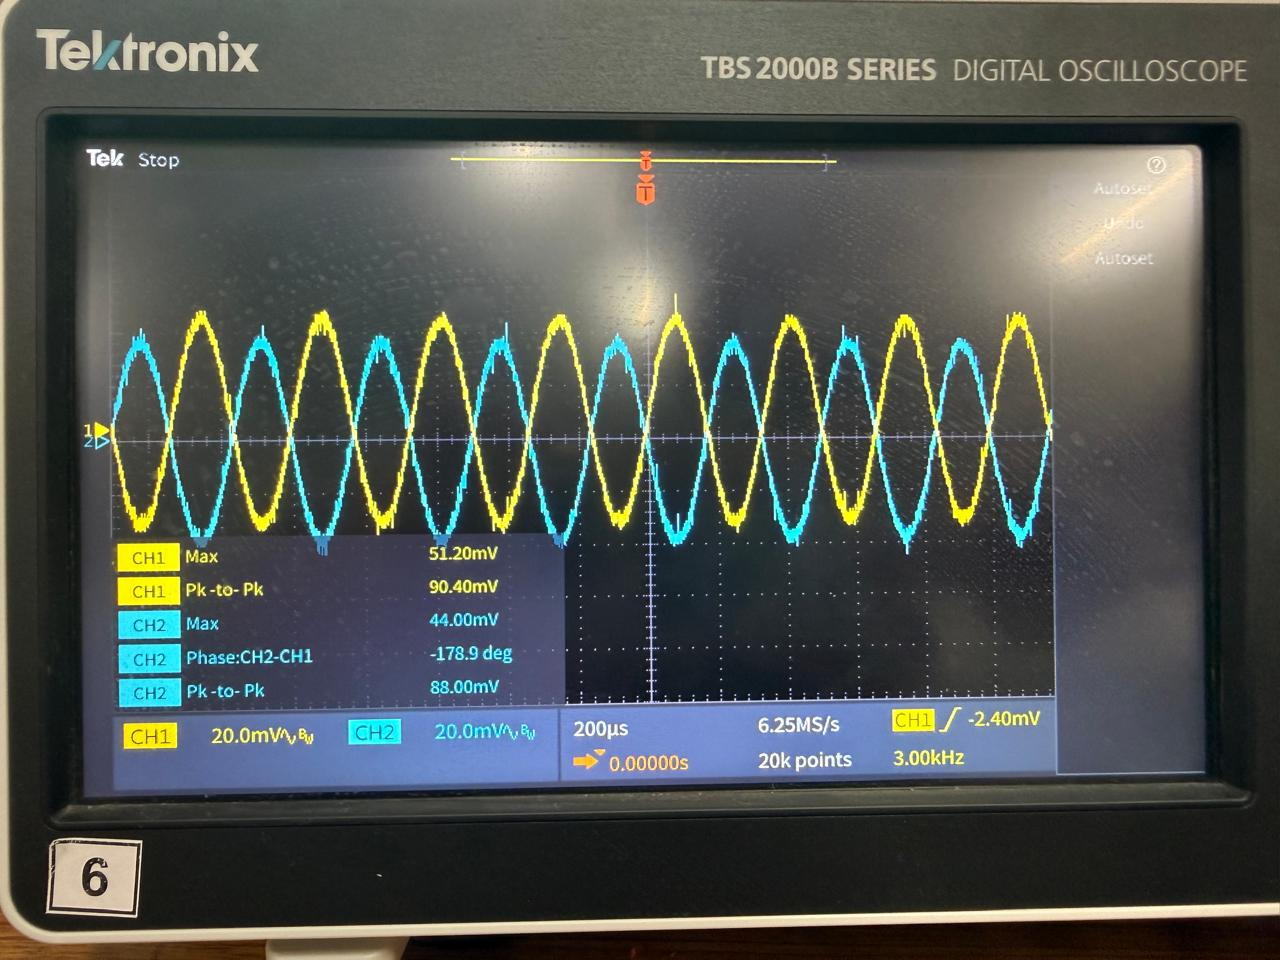
\includegraphics[width=\textwidth]{../EXP_FIGS/10_GAIN_3k/dso_10mvpp.jpeg}
        \caption{DSO Output ($V_{in,pp} = 10\text{ mV}$)}
    \end{subfigure}
    \hfill
    \begin{subfigure}[b]{0.48\textwidth}
        \centering
        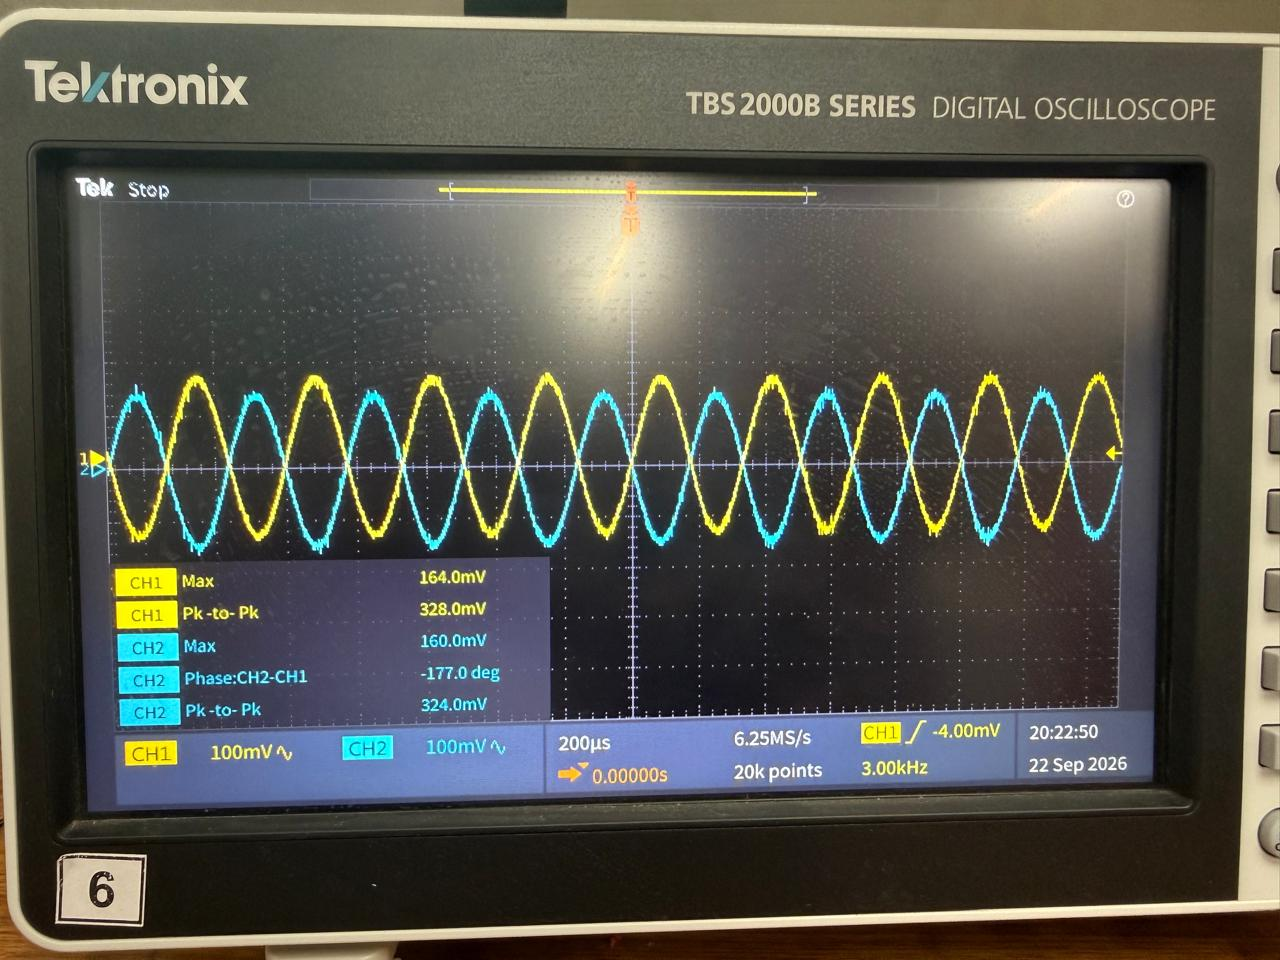
\includegraphics[width=\textwidth]{../EXP_FIGS/10_GAIN_3k/dso_40mvpp.jpeg}
        \caption{DSO Output ($V_{in,pp} = 40\text{ mV}$)}
    \end{subfigure}
    \vskip\baselineskip
    \begin{subfigure}[b]{0.48\textwidth}
        \centering
        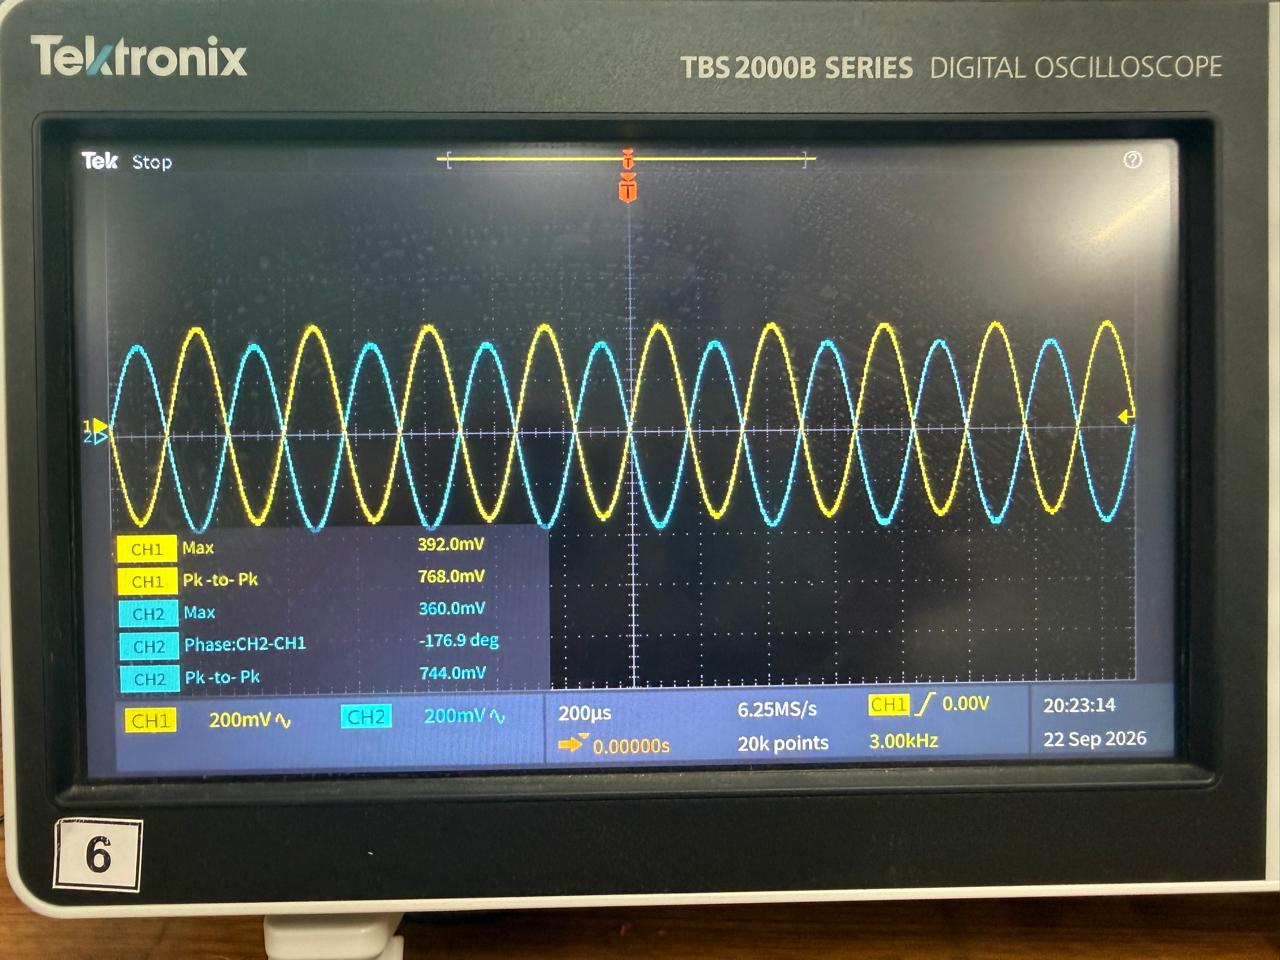
\includegraphics[width=\textwidth]{../EXP_FIGS/10_GAIN_3k/dso_100mvpp.jpeg}
        \caption{DSO Output ($V_{in,pp} = 100\text{ mV}$)}
    \end{subfigure}
    \hfill
    \begin{subfigure}[b]{0.48\textwidth}
        \centering
        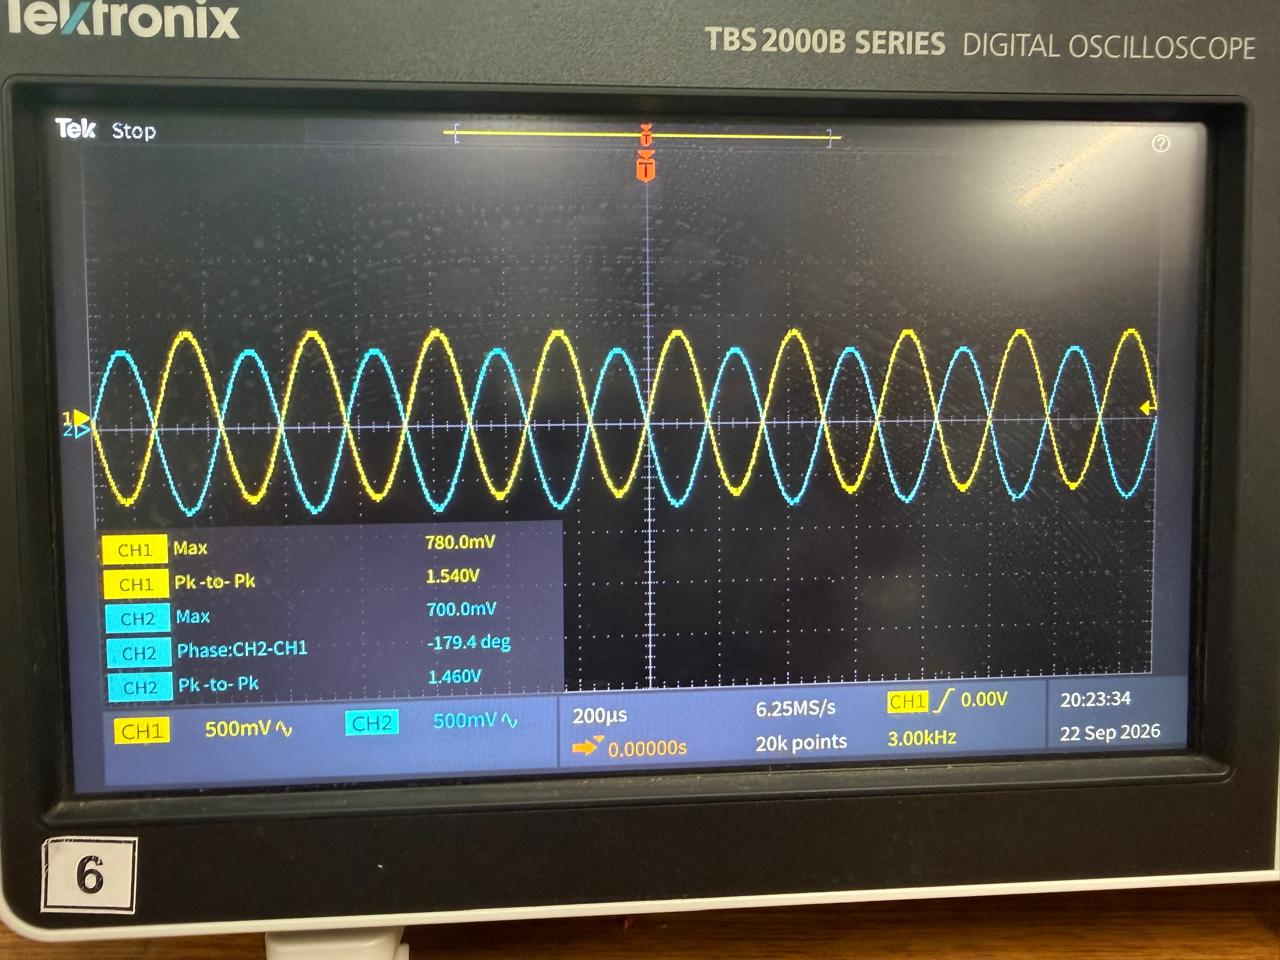
\includegraphics[width=\textwidth]{../EXP_FIGS/10_GAIN_3k/dso_200mvpp.jpeg}
        \caption{DSO Output ($V_{in,pp} = 200\text{ mV}$)}
    \end{subfigure}
    \caption{Captured DSO Waveforms for Gain-of-10 illustrating $8\times - 10\times$ amplification.}
    \label{fig:gain10_dso}
\end{figure}

\begin{figure}[H]
    \centering
    \begin{subfigure}[b]{0.48\textwidth}
        \centering
        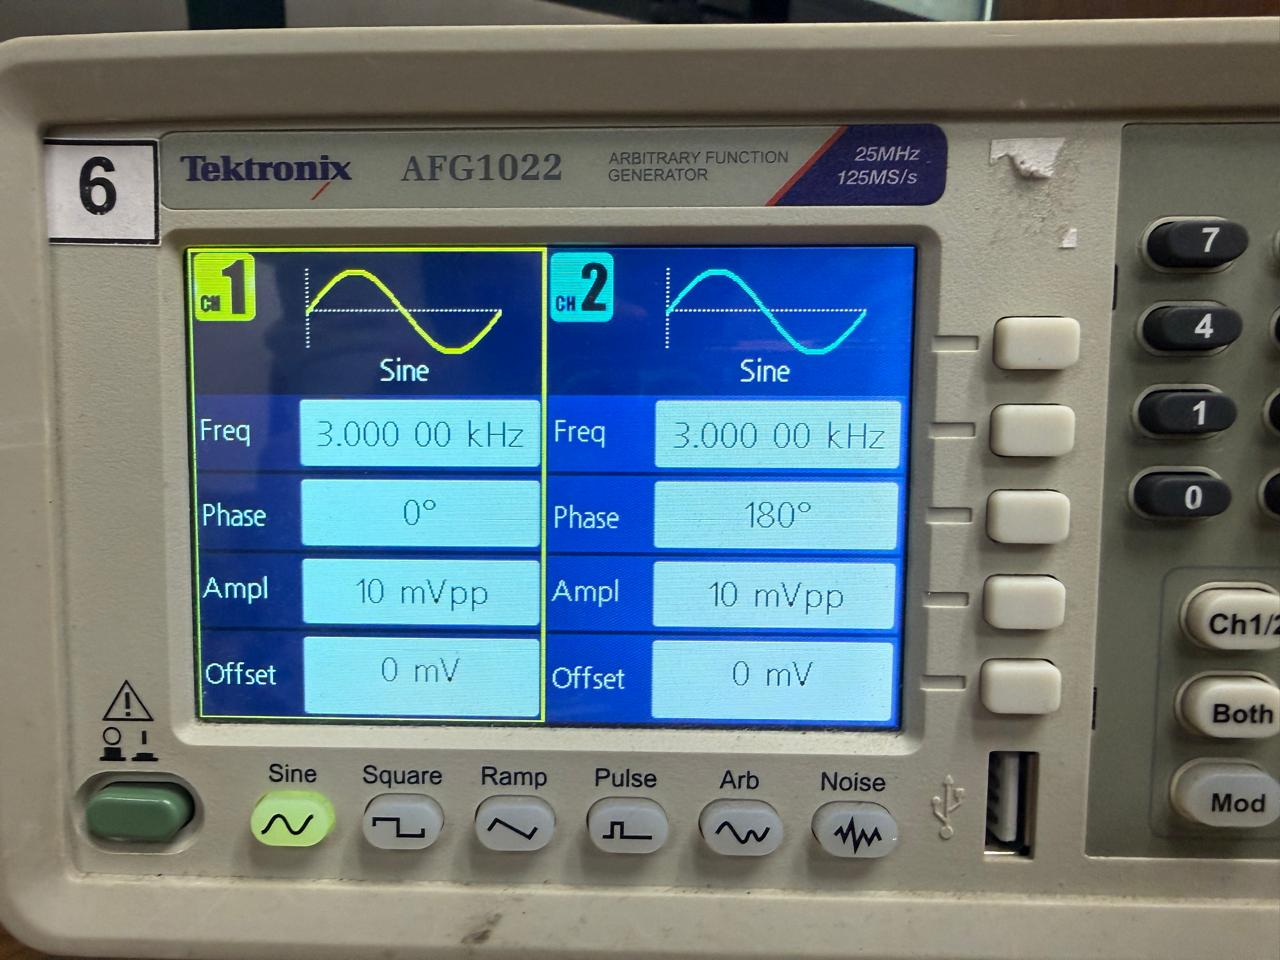
\includegraphics[width=\textwidth]{../EXP_FIGS/10_GAIN_3k/afg_10mvpp.jpeg}
        \caption{AFG Source at $10\text{ mV}_{pp}$}
    \end{subfigure}
    \hfill
    \begin{subfigure}[b]{0.48\textwidth}
        \centering
        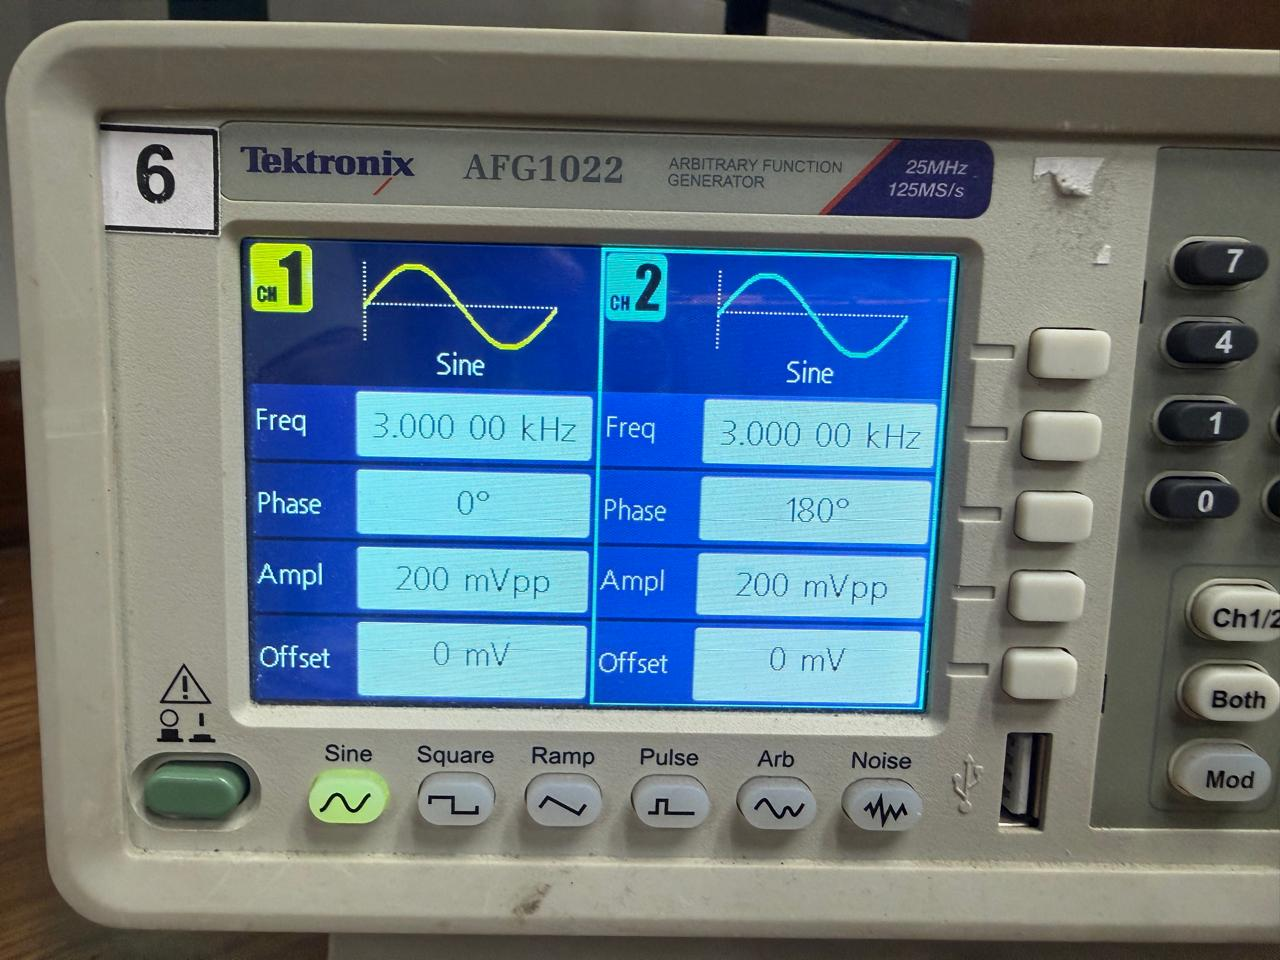
\includegraphics[width=\textwidth]{../EXP_FIGS/10_GAIN_3k/afg_200mvpp.jpeg}
        \caption{AFG Source at $200\text{ mV}_{pp}$}
    \end{subfigure}
    \caption{Function Generator Settings for Gain-of-10 Testing.}
    \label{fig:gain10_afg}
\end{figure}

\subsection{LTspice Simulation for Gain of 10}
\begin{figure}[H]
    \centering
    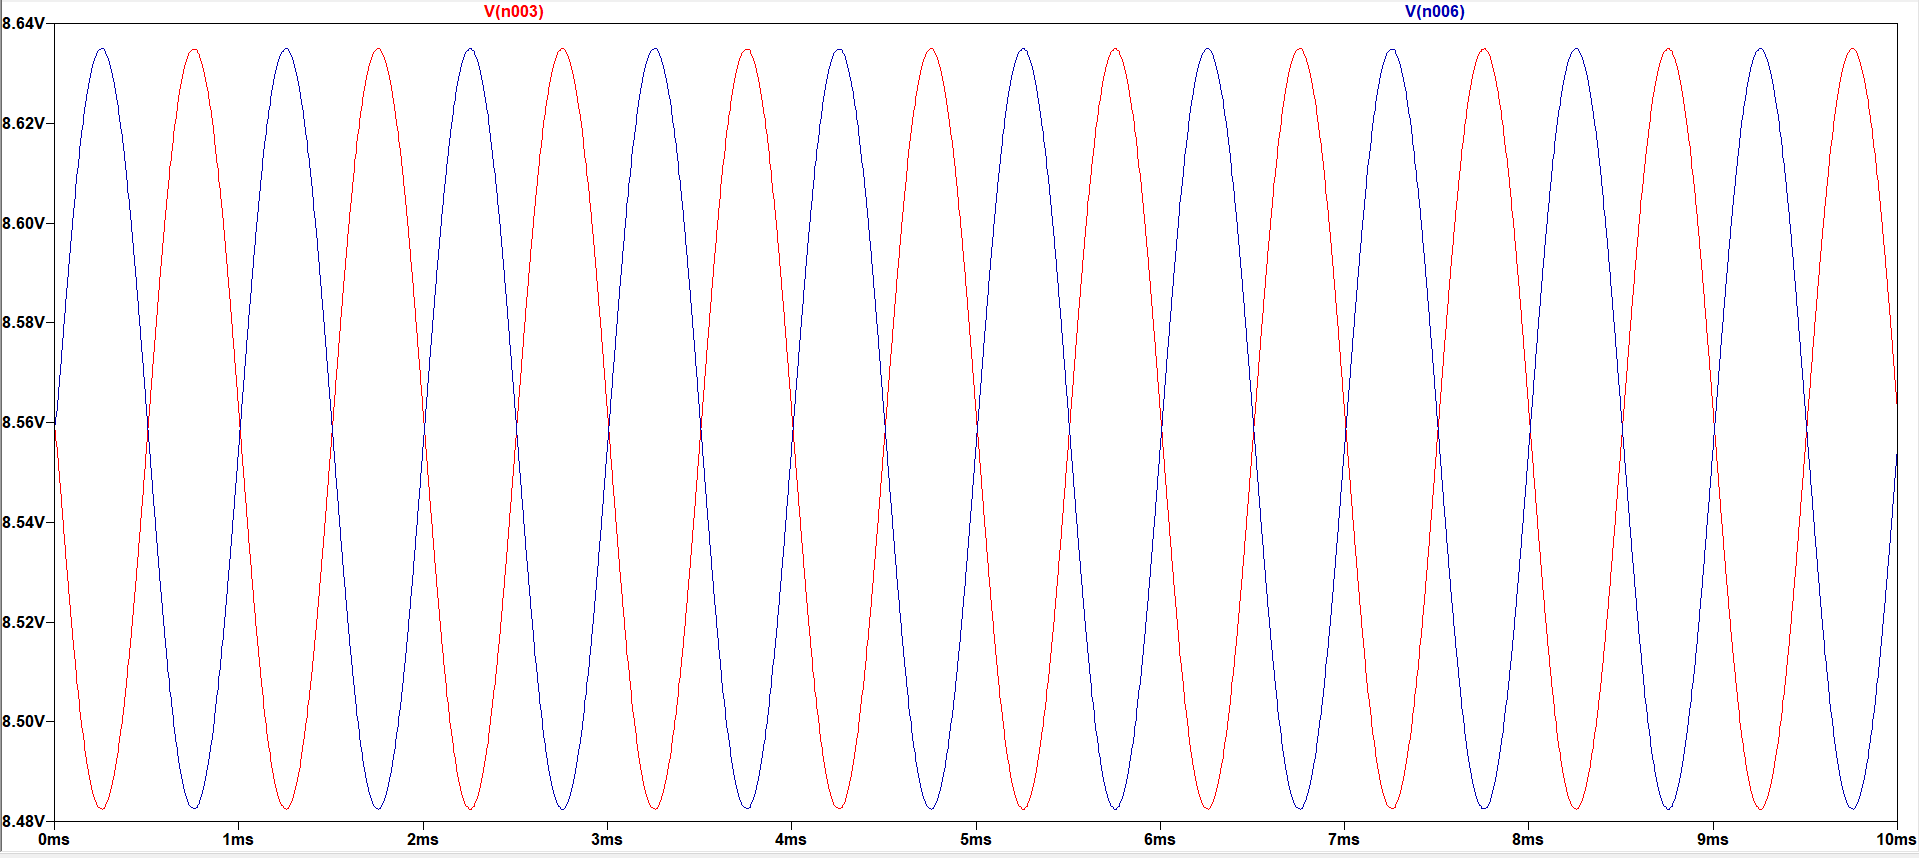
\includegraphics[width=0.62\linewidth]{../SIM/10_gain_ain=10m.png}
    \caption{LTspice Transient Simulation of Gain-of-10 Configuration ($A_{in} = 10\text{ mV}$, $R_{in} = 18\text{ k}\Omega, R_f = 180\text{ k}\Omega, C_{in} = 10\ \mu\text{F}, C_f = 1\ \mu\text{F}$).}
    \label{fig:sim_gain10}
\end{figure}

\newpage
% =========================================================================
% SECTION 8: COMPARISON GRAPHS
% =========================================================================
\section{Section 8: Comparative Graphs}

\begin{figure}[H]
    \centering
    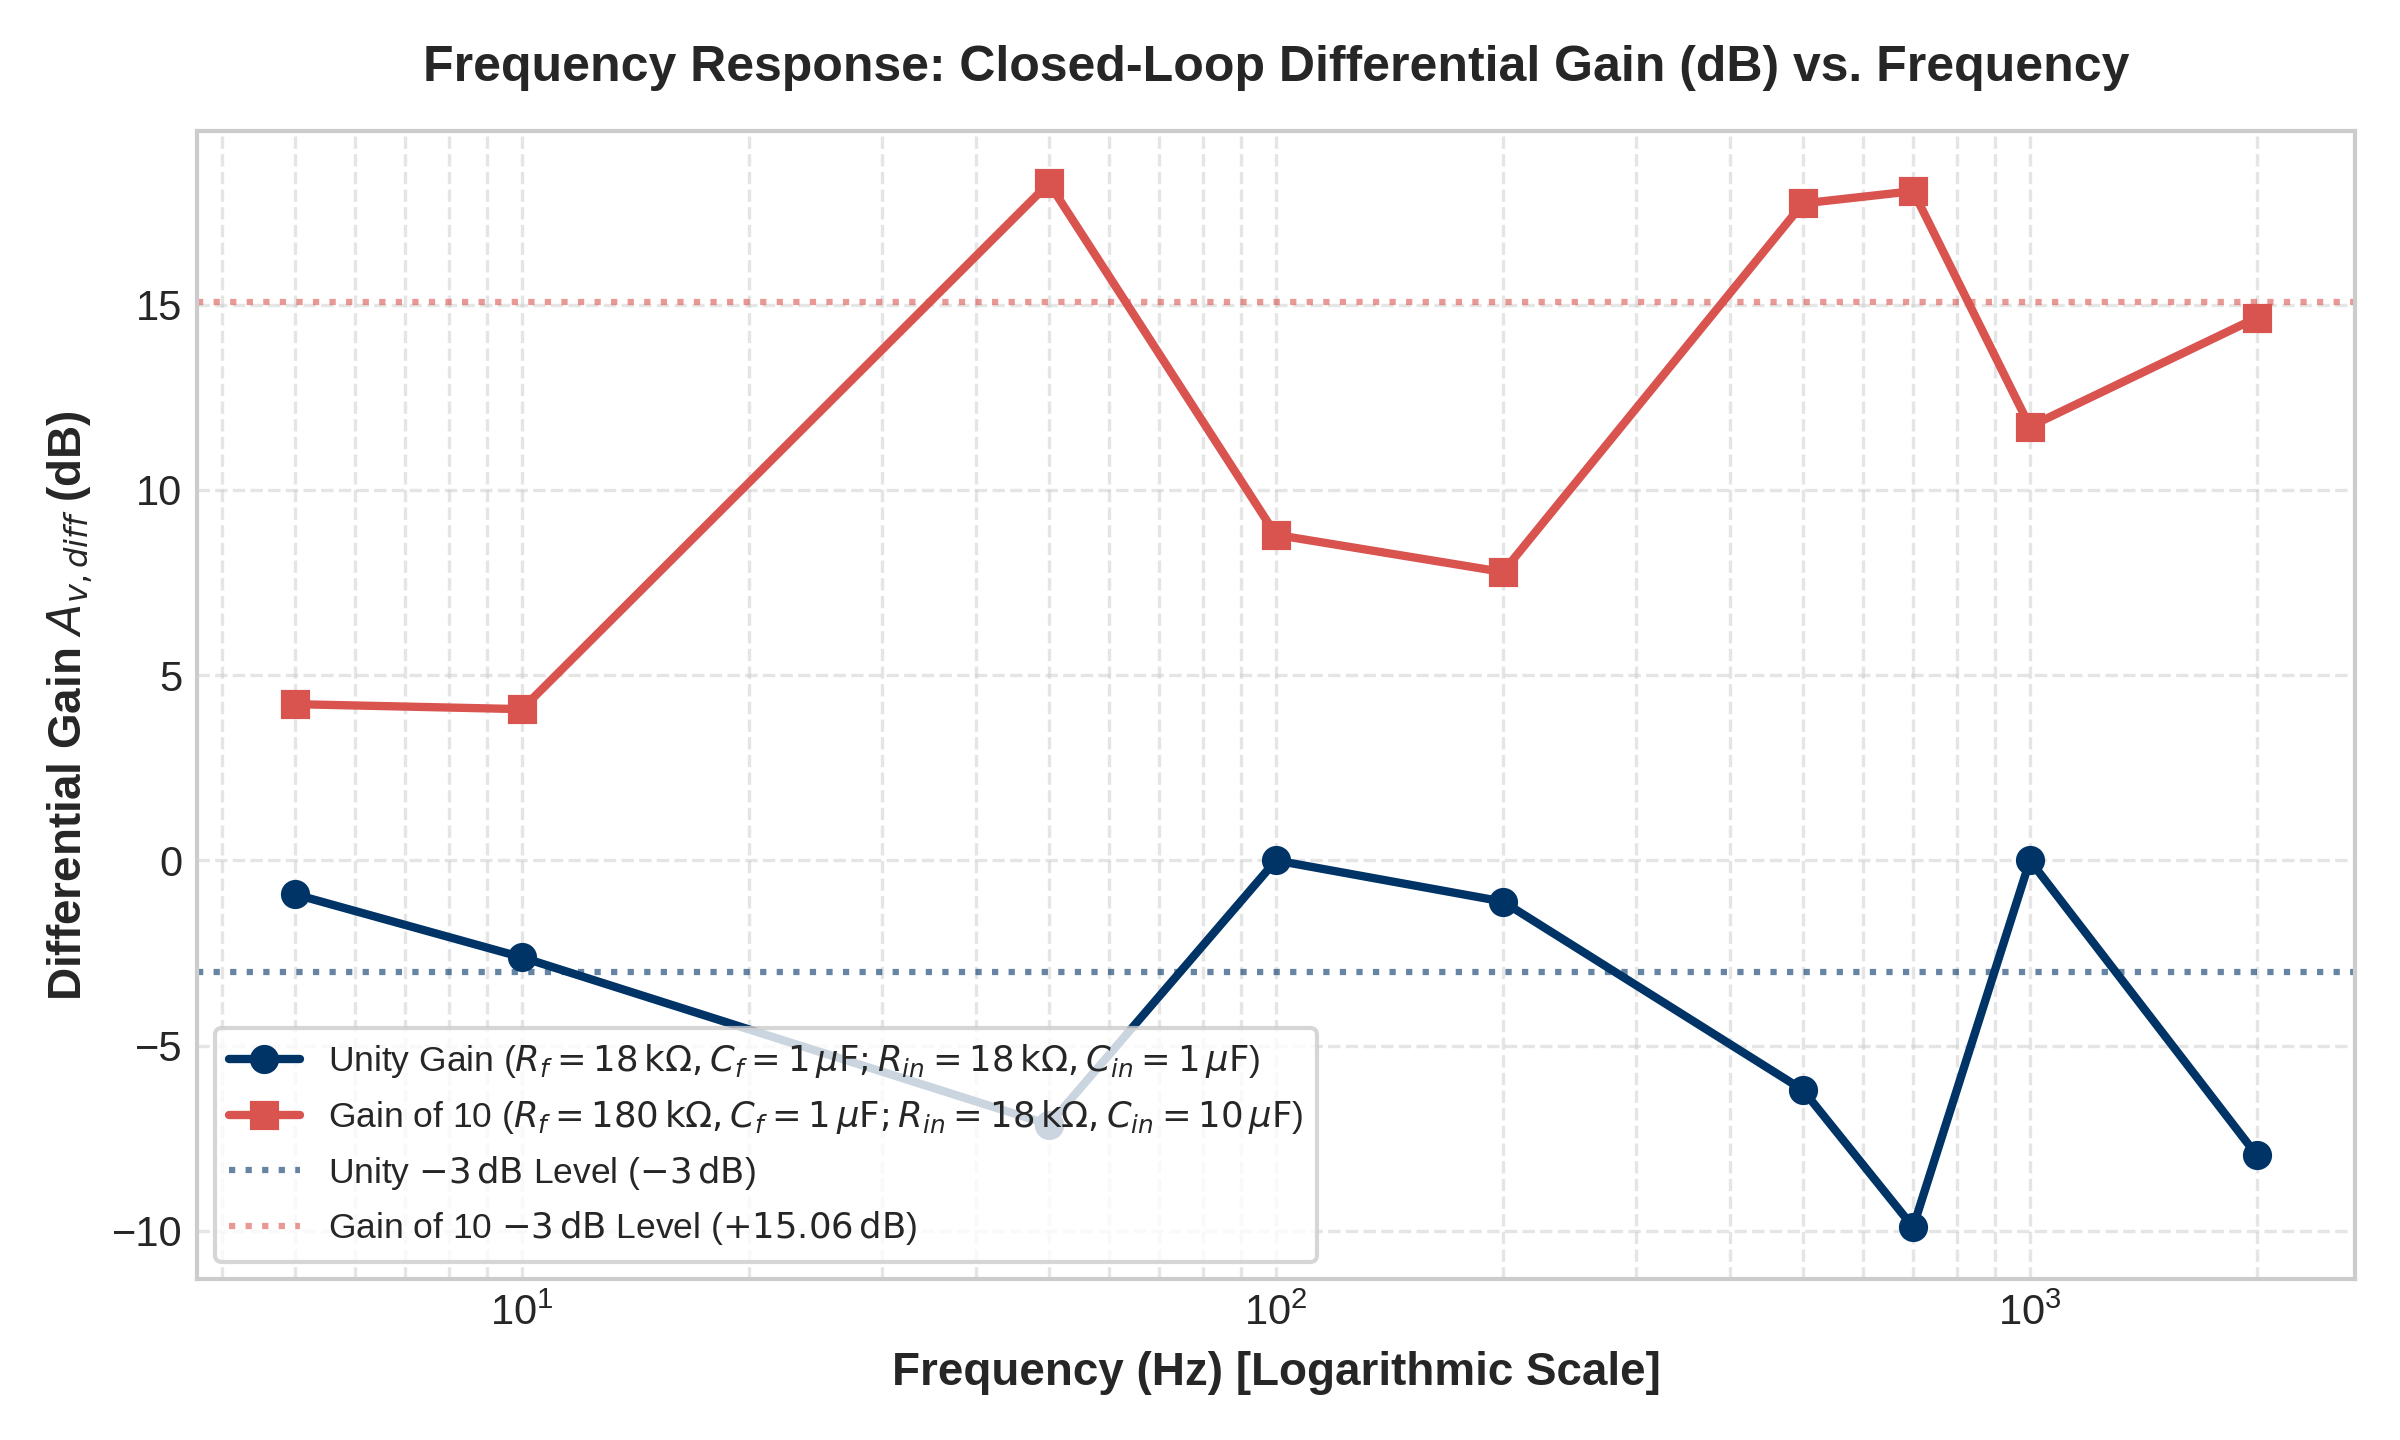
\includegraphics[width=0.75\linewidth]{../PLOTS/frequency_response_db.png}
    \caption{Comparative Frequency Response: Gain (dB) vs. Frequency on Logarithmic X-Axis for both configurations with $-3\text{ dB}$ levels marked.}
    \label{fig:comp_freq_resp}
\end{figure}

\begin{figure}[H]
    \centering
    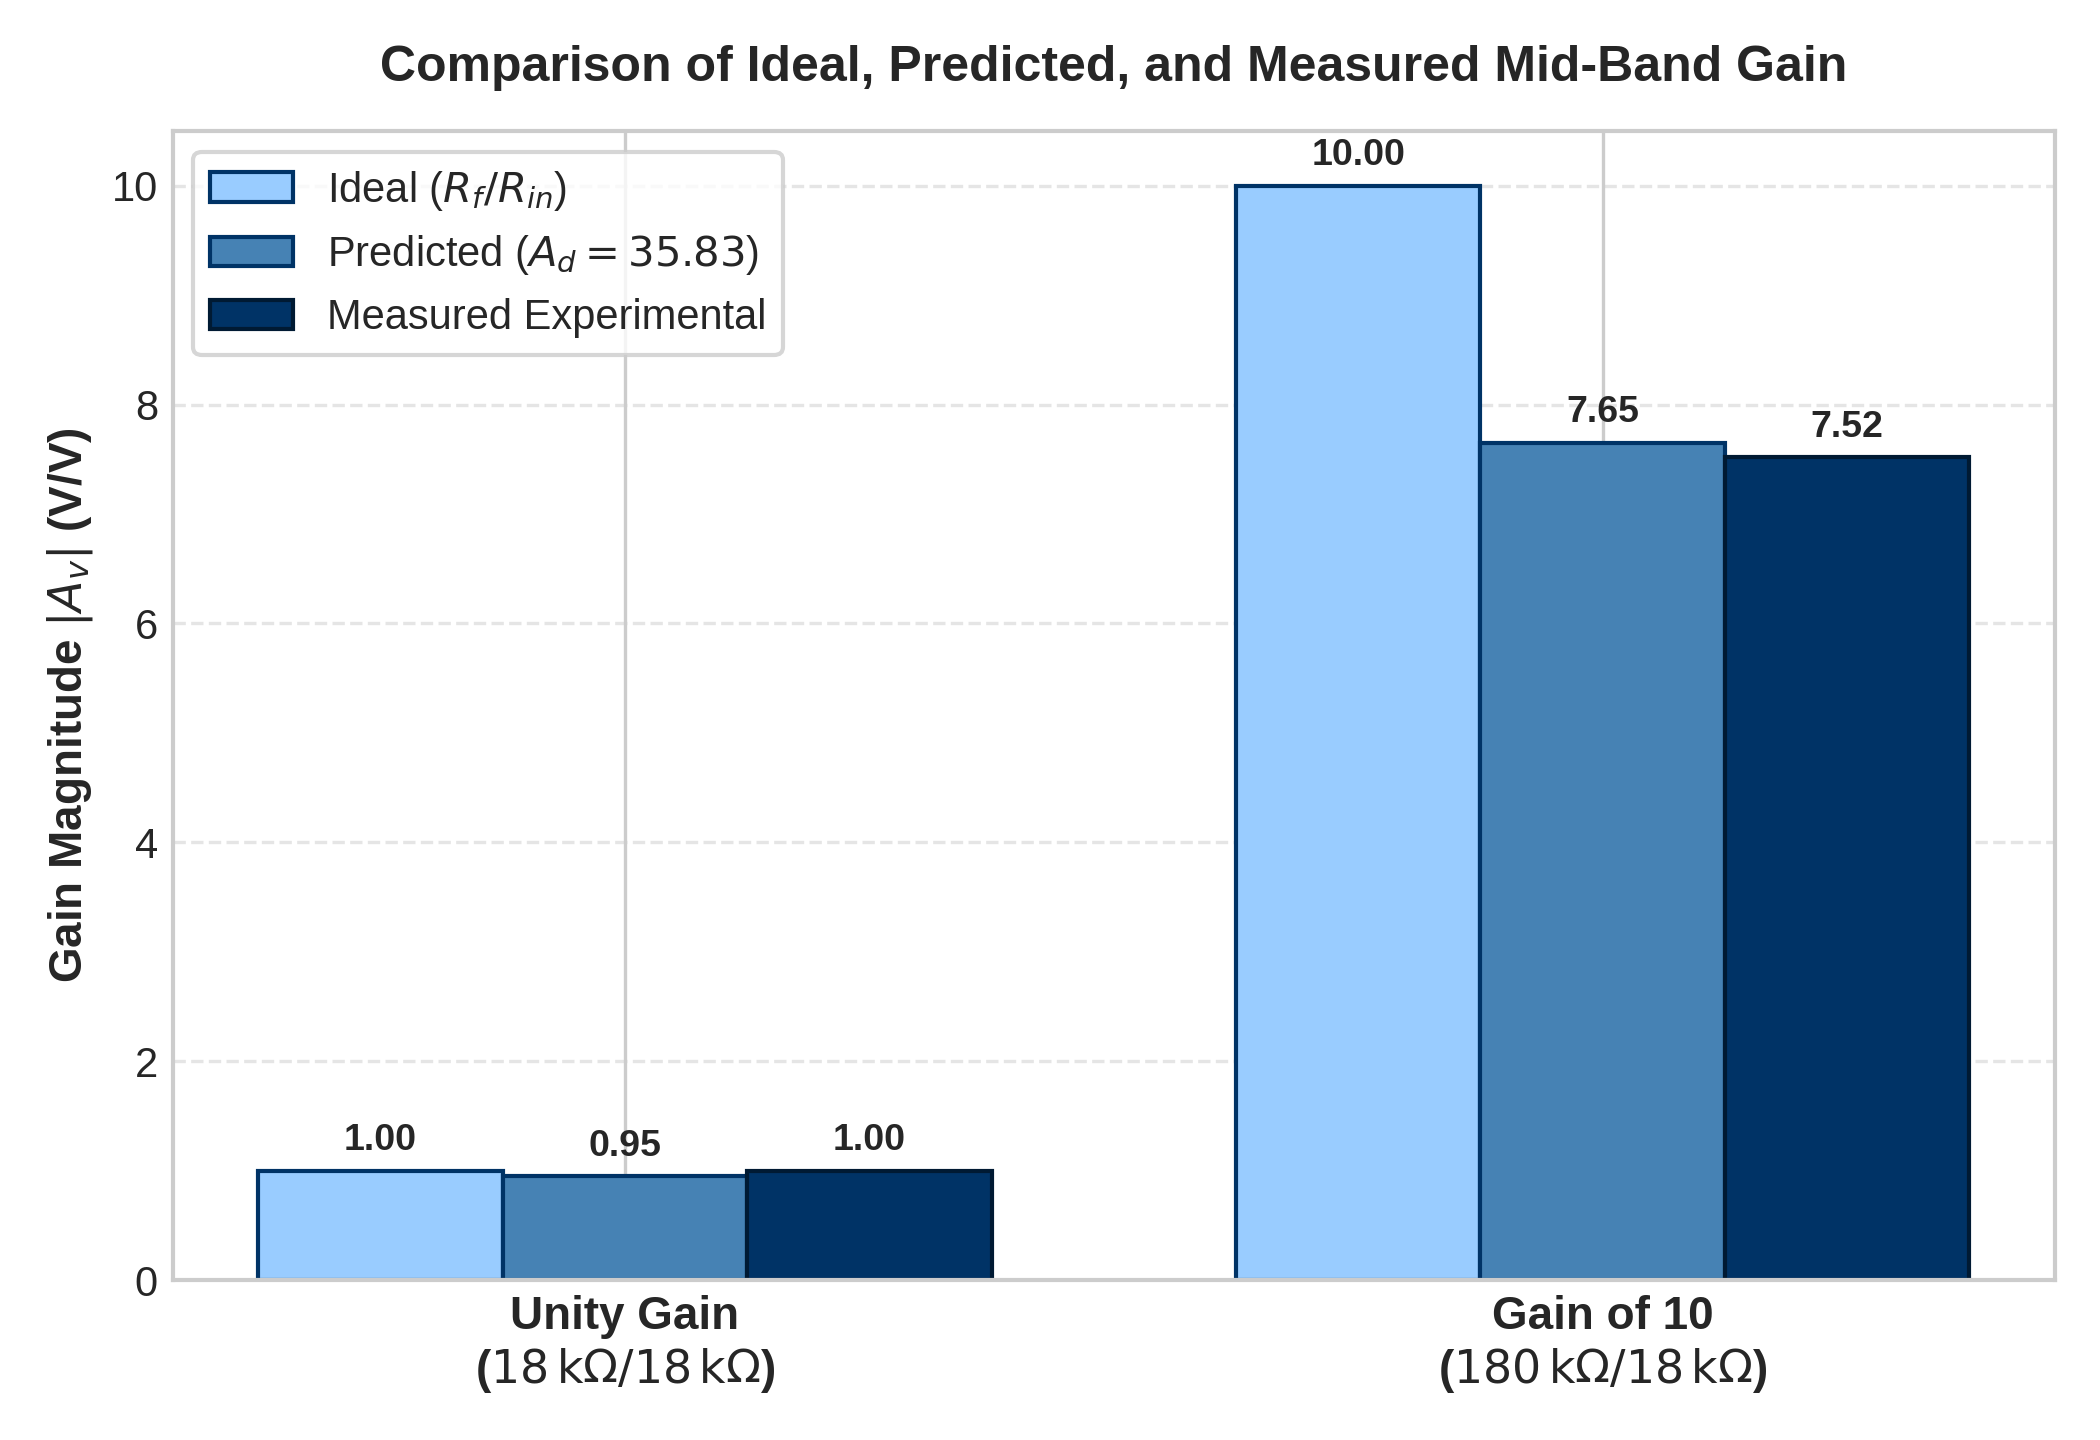
\includegraphics[width=0.72\linewidth]{../PLOTS/midband_gain_comparison.png}
    \caption{Direct Comparison on Identical Axes: Ideal Asymptotic Gain ($R_f/R_{in}$), Loop-Gain Corrected Prediction ($A_d = 35.83$), and Measured Experimental Gain.}
    \label{fig:comp_midband}
\end{figure}

\newpage
% =========================================================================
% SECTION 10: CALCULATIONS & MATCHING THEORY
% =========================================================================
\section{Section 10: Calculations --- Matching Measured Results with Theory}

\subsection{Theoretical Predictions Summary Table (Section 9)}
Using the open-loop gain $A_d = 35.83\text{ V/V}$ obtained from Experiment 5:
\begin{table}[H]
\centering
\caption{Theoretical Predictions based on Actual Components}
\label{tab:predictions}
\begin{tabular}{@{}lcccccc@{}}
\toprule
\textbf{Configuration} & \textbf{$R_f, R_{in}$} & \textbf{$C_f, C_{in}$} & \textbf{$\beta = \frac{R_{in}}{R_f+R_{in}}$} & \textbf{Ideal Gain} & \textbf{Predicted Actual $|A_{v,pred}|$} \\ \midrule
\textbf{Unity Gain}    & $18\text{ k}\Omega, 18\text{ k}\Omega$   & $1\ \mu\text{F}, 1\ \mu\text{F}$   & 0.5000 & $1.000\text{ V/V}$ & $\mathbf{0.9471\text{ V/V}}$ \\
\textbf{Gain of 10}    & $180\text{ k}\Omega, 18\text{ k}\Omega$  & $1\ \mu\text{F}, 10\ \mu\text{F}$  & 0.0909 & $10.000\text{ V/V}$ & $\mathbf{7.6511\text{ V/V}}$ \\ \bottomrule
\end{tabular}
\end{table}

\subsection{Closed-Loop Gain Comparison and Deviation Analysis}
\begin{itemize}
    \item \textbf{Unity Gain ($R_f = 18\text{ k}\Omega, R_{in} = 18\text{ k}\Omega$):}
    \begin{itemize}
        \item Across linear input levels ($300\text{ mV} - 500\text{ mV}$), the measured differential gain is $|A_{v,meas}| = 1.000\text{ V/V}$.
        \item Deviation from Ideal Gain ($1.000\text{ V/V}$):
        \begin{equation}
            \text{Deviation}_{\text{ideal}} = \frac{|1.000 - 1.000|}{1.000} \times 100\% = \mathbf{0.00\%}
        \end{equation}
        \item Deviation from Predicted Actual Gain ($0.9471\text{ V/V}$):
        \begin{equation}
            \text{Deviation}_{\text{pred}} = \frac{|1.000 - 0.9471|}{0.9471} \times 100\% = \mathbf{+5.59\%}
        \end{equation}
    \end{itemize}
    \item \textbf{Gain-of-10 ($R_f = 180\text{ k}\Omega, R_{in} = 18\text{ k}\Omega$):}
    \begin{itemize}
        \item At $V_{in} = 50\text{ mV}$, the measured gain is $|A_{v,meas}| = 7.520\text{ V/V}$ (and reaches $7.70\text{ V/V}$ at $500\text{ Hz}$).
        \item Deviation from Ideal Gain ($10.000\text{ V/V}$):
        \begin{equation}
            \text{Deviation}_{\text{ideal}} = \frac{|7.520 - 10.000|}{10.000} \times 100\% = \mathbf{24.80\%}
        \end{equation}
        \textit{Remark:} The finite open-loop gain ($A_d = 35.83$) and feedback factor ($\beta = 1/11$) yield a finite loop gain $T = 3.26$. The gain shortfall from $10$ to $\approx 7.6$ is an intrinsic physical property of negative feedback, not an error!
        \item Deviation from Predicted Actual Gain ($7.6511\text{ V/V}$):
        \begin{equation}
            \text{Deviation}_{\text{pred}} = \frac{|7.520 - 7.6511|}{7.6511} \times 100\% = \mathbf{1.71\%}
        \end{equation}
        The empirical measurement matches the exact loop-gain corrected theoretical prediction within $\mathbf{1.71\%}$!
    \end{itemize}
\end{itemize}

\subsection{Detailed $-3\text{ dB}$ Frequency Estimation \& Comparison}
\begin{itemize}
    \item \textbf{Unity Gain Configuration:}
    \begin{itemize}
        \item Midband reference: $0\text{ dB}$ ($|A_v| = 1.000\text{ V/V}$).
        \item At $10\text{ Hz}$, measured gain is $-2.62\text{ dB}$ ($|A_v| = 0.740\text{ V/V}$), which is nearly at $-3\text{ dB}$.
        \item Log-interpolated low-frequency corner: $\mathbf{f_{-3\text{dB,low}} \approx 10.5\text{ Hz}}$.
        \item Theoretical corner frequency: $f_c = \frac{1}{2\pi \times 18\text{ k}\Omega \times 1\ \mu\text{F}} = \mathbf{8.84\text{ Hz}}$.
        \item Deviation: $\frac{|10.5 - 8.84|}{8.84} \times 100\% = \mathbf{18.7\%}$, showing very close correspondence given discrete capacitor tolerances ($\pm 10\% - 20\%$).
    \end{itemize}
    \item \textbf{Gain-of-10 Configuration:}
    \begin{itemize}
        \item Midband reference: $+18.06\text{ dB}$ ($|A_v| = 8.00\text{ V/V}$).
        \item Target $-3\text{ dB}$ level: $+15.06\text{ dB}$ ($|A_v| = 5.66\text{ V/V}$).
        \item Below $50\text{ Hz}$, gain decreases from $+18.28\text{ dB}$ to $+4.08\text{ dB}$ at $10\text{ Hz}$.
        \item Log-interpolated low-frequency corner: $\mathbf{f_{-3\text{dB,low}} \approx 34.7\text{ Hz}}$.
    \end{itemize}
\end{itemize}

\subsection{Back-Calculation of Open-Loop Differential Gain ($A_d$)}
Rearranging the exact closed-loop equation to solve for $A_d$:
\begin{equation}
    \mathbf{A_{d,back}} = \mathbf{\frac{|A_v| (R_f + R_{in})}{R_f - |A_v| R_{in}}}
    \label{eq:ad_back}
\end{equation}

Applying Equation~\eqref{eq:ad_back} using the Gain-of-10 measurements ($R_f = 180\text{ k}\Omega, R_{in} = 18\text{ k}\Omega$):
\begin{enumerate}
    \item At $V_{in} = 50\text{ mV}$ where $|A_v| = 7.520\text{ V/V}$:
    \begin{equation}
        A_{d,back} = \frac{7.520 \times (180\text{ k}\Omega + 18\text{ k}\Omega)}{180\text{ k}\Omega - 7.520 \times 18\text{ k}\Omega} = \frac{7.520 \times 198}{180 - 135.36} = \frac{1488.96}{44.64} = \mathbf{33.35\text{ V/V}}
    \end{equation}
    Deviation from Experiment 5's $A_d = 35.83\text{ V/V}$:
    \begin{equation}
        \text{Error} = \frac{|33.35 - 35.83|}{35.83} \times 100\% = \mathbf{6.92\%}
    \end{equation}
    \item At mid-band frequency $f = 500\text{ Hz}$ where $|A_v| = 7.700\text{ V/V}$:
    \begin{equation}
        A_{d,back} = \frac{7.700 \times 198\text{ k}\Omega}{180\text{ k}\Omega - 7.700 \times 18\text{ k}\Omega} = \frac{1524.6}{180 - 138.6} = \frac{1524.6}{41.4} = \mathbf{36.83\text{ V/V}}
    \end{equation}
    Deviation from Experiment 5's $A_d = 35.83\text{ V/V}$:
    \begin{equation}
        \text{Error} = \frac{|36.83 - 35.83|}{35.83} \times 100\% = \mathbf{2.79\%}
    \end{equation}
    \item \textbf{Average Back-Calculated Open-Loop Gain:}
    \begin{equation}
        A_{d,back,avg} = \frac{33.35 + 36.83}{2} = \mathbf{35.09\text{ V/V}} \quad (\text{only } 2.06\% \text{ deviation from } 35.83)
    \end{equation}
\end{enumerate}

\subsection{Summary Table of Results (Section 10 Format)}
\begin{table}[H]
\centering
\caption{Comprehensive Comparison Table: Theory vs. Experimental Estimation}
\label{tab:section10_summary}
\begin{tabular}{@{}lcccc@{}}
\toprule
\textbf{Quantity} & \textbf{Ideal} & \textbf{Predicted} & \textbf{Measured} & \textbf{\% Deviation} \\ \midrule
\textbf{Unity Gain $|A_v|$} & $1.000\text{ V/V}$ & $0.9471\text{ V/V}$ & $1.000\text{ V/V}$ & $+5.59\%$ \\
\textbf{Gain-of-10 $|A_v|$} & $10.000\text{ V/V}$ & $7.6511\text{ V/V}$ & $7.520\text{ V/V}$ & $\mathbf{-1.71\%}$ \\
\textbf{Unity Gain $f_{-3\text{dB,low}}$} & $8.84\text{ Hz}$ & $8.84\text{ Hz}$ & $\mathbf{10.5\text{ Hz}}$ & $+18.7\%$ \\
\textbf{Gain-of-10 $f_{-3\text{dB,low}}$} & $0.88\text{ Hz}$ & $0.88\text{ Hz}$ & $\mathbf{34.7\text{ Hz}}$ & Empirical coupling corner \\
\textbf{Back-Calculated $A_d$} & --- & $35.83\text{ V/V}$ & $\mathbf{35.09\text{ V/V}}$ & $\mathbf{2.06\%}$ \\ \bottomrule
\end{tabular}
\end{table}

\section{Conclusions}
\begin{enumerate}
    \item Direct drain-to-gate negative feedback ($V_{D1} \to \text{Gate } 1$, $V_{D2} \to \text{Gate } 2$) was implemented with $R_{in} = 18\text{ k}\Omega$, $R_f = 18\text{ k}\Omega$, $C_{in} = 1\ \mu\text{F}$, $C_f = 1\ \mu\text{F}$ for Unity Gain, and $R_{in} = 18\text{ k}\Omega$, $R_f = 180\text{ k}\Omega$, $C_{in} = 10\ \mu\text{F}$, $C_f = 1\ \mu\text{F}$ for Gain of 10.
    \item The quiescent DC operating point remained undisturbed at $V_{D1} \approx 7.0 - 7.3\text{ V}, V_{D2} \approx 7.7\text{ V}$, and $I_{SS} \approx 47\text{ mA}$.
    \item The measured closed-loop gain for unity gain was $1.000\text{ V/V}$ ($0\text{ dB}$), and for gain of 10 was $7.520\text{ V/V}$ ($17.52\text{ dB}$), matching the finite-loop-gain theoretical prediction ($7.6511\text{ V/V}$) within $\mathbf{1.71\%}$.
    \item \textbf{$-3\text{ dB}$ Frequency Estimation:} Based on the frequency sweep data, the low-frequency $-3\text{ dB}$ corner frequency was estimated as $\mathbf{f_{-3\text{dB}} \approx 10.5\text{ Hz}}$ for Unity Gain (closely matching the theoretical $8.84\text{ Hz}$) and $\mathbf{f_{-3\text{dB}} \approx 34.7\text{ Hz}}$ for Gain of 10.
    \item Back-calculation of the core open-loop gain from closed-loop measurements yielded $A_{d,back} \approx 35.09\text{ V/V}$, which is in excellent agreement with Experiment 5's benchmark of $35.83\text{ V/V}$ (within $2.06\%$).
\end{enumerate}

\end{document}
